%% ====================================================================
%%  Systemic Risk as Geometry: A Unified Theory of Financial Instability,
%%  Detection, and Adaptive Stabilisation
%%
%%  Draft v0.1  —  February 2026
%% ====================================================================
\documentclass[11pt]{article}

%% ---- Geometry -------------------------------------------------------
\usepackage[margin=1.15in, top=1.1in, bottom=1.2in]{geometry}

%% ---- Mathematics ---------------------------------------------------
\usepackage{amsmath, amsthm, amssymb, mathtools}
\usepackage{bm}          % bold math symbols
\usepackage{bbm}         % blackboard bold for 1

%% ---- References / Hyperlinks ---------------------------------------
\usepackage[colorlinks=true, linkcolor=blue!70!black,
            citecolor=blue!60!black, urlcolor=blue!60!black]{hyperref}
\usepackage[numbers, sort&compress]{natbib}

%% ---- Fonts / Layout ------------------------------------------------
\usepackage{microtype}
\usepackage{booktabs, tabularx, multirow}
\usepackage{graphicx}
\usepackage{xcolor}
\usepackage{tcolorbox}
\tcbuselibrary{skins, breakable}

%% ---- Algorithms ----------------------------------------------------
\usepackage{algorithm, algpseudocode}

%% ---- Appendix ------------------------------------------------------
\usepackage[toc, page]{appendix}

%% ====================================================================
%%  Theorem Environments
%% ====================================================================
\newtheorem{theorem}{Theorem}[section]
\newtheorem{lemma}[theorem]{Lemma}
\newtheorem{proposition}[theorem]{Proposition}
\newtheorem{corollary}[theorem]{Corollary}
\newtheorem{definition}[theorem]{Definition}
\newtheorem{remark}[theorem]{Remark}
\newtheorem{assumption}{Assumption}
\renewcommand{\theassumption}{E\arabic{assumption}}

\theoremstyle{definition}
\newtheorem{example}[theorem]{Example}

%% ====================================================================
%%  Macros
%% ====================================================================
\DeclareMathOperator{\sym}{sym}
\DeclareMathOperator{\erf}{erf}
\DeclareMathOperator*{\argmin}{arg\,min}
\newcommand{\R}{\mathbb{R}}
\newcommand{\E}{\mathbb{E}}
\newcommand{\Xst}{X^{\star}}
\newcommand{\grad}{\nabla}
\newcommand{\Ebs}{E_{\mathrm{BS}}}
\newcommand{\Cman}{\mathcal{C}}
\newcommand{\Lpair}{L_{\mathrm{pair}}}
\newcommand{\lmax}{\lambda_{\max}}
\newcommand{\lmin}{\lambda_{\min}}
\newcommand{\norm}[1]{\left\|#1\right\|}
\newcommand{\inner}[2]{\left\langle #1,\, #2\right\rangle}
\newcommand{\costheta}{\cos\theta}
\newcommand{\ddt}{\tfrac{d}{dt}}

%% ====================================================================
%%  Title / Authors
%% ====================================================================
\title{%
  \textbf{Systemic Risk as Geometry}\\[4pt]
  \large A Unified Theory of Financial Instability, Detection,
         and Adaptive Stabilisation
}
\author{%
  [Author redacted for review]
}
\date{Draft: \today \\ \small\textit{Subject to revision — not for circulation}}

%% ====================================================================
\begin{document}
\maketitle

\begin{abstract}
We establish a geometric framework linking the statistical structure of financial
blind spots to the Lyapunov energy of networked agent dynamics.  The Blind-Spot
Detection Theory (BSDT) deviation operators---four complementary channels
($\delta_C$, $\delta_G$, $\delta_A$, $\delta_T$) calibrated solely on
normal-period data---generate a functional $\Ebs(X)$ whose gradient is
\emph{anti-aligned} with the gravitational restoring force on real data
(empirical $\costheta = -0.335$ over 140 quarters of FDIC call reports).
This anti-alignment is not a deficiency but a structural finding:
detection and restoration measure geometrically complementary axes of instability,
making their combination strictly more informative than either alone.
We prove three formal results.
(i)~\textbf{Theorem~C} (equivalence): $\Ebs$ and the GravityEngine potential $\Phi$
are equivalent Lyapunov functions on every compact sublevel set.
(ii)~\textbf{Theorem~2} (phase transition): a spectral radius criterion identifies a
critical manifold $\Cman$ above which no bounded constant coupling stabilises the
system, but state-adaptive $\gamma(X)$ does.
(iii)~\textbf{Theorem~OR2} (optimal policy): the adaptive damping law
$\gamma^*(X) \approx E(X)/(E(X)+\theta)$ solves an infinite-horizon stochastic control
problem with intervention cost $\kappa$ in closed form.
We validate the framework on exclusively real data at three levels of aggregation:
(a)~140~quarters of FDIC Statistics on Depository Institutions call reports
(1990--2024, $N=7$ institution types, $d=6$ CAMELS-adjacent features);
(b)~an individual bank-level panel ($N=30$ largest U.S.\ commercial banks,
$T=140$, $d=5$); and (c)~a cross-border G-SIB panel ($N=20$ Global Systemically
Important Banks, $T=76$ quarters from 2005--2023, $d=5$; U.S.\ banks from FDIC,
non-U.S.\ banks from World Bank GFDD and ECB MIR---no synthetic data).
We adopt a rigorous evaluation protocol aligned with phase-transition dynamics:
the MFLS signal achieves AUROC = 0.87 on the cross-border panel (Full BSDT
variant) and 0.81 at the bank level, fires its GFC alarm 6~quarters before
Lehman at every scale, and passes three pre-registered robustness checks
(alternate normal period, rolling refit, leave-one-crisis-out threshold
calibration).
We report Granger causality results honestly: all five MFLS variants fail at
$\alpha = 0.10$ on domestic data, confirming the phase-transition thesis---crises
are threshold crossings, not linearly predictable trends.  On the cross-border
G-SIB panel, however, threshold Granger causality \emph{passes} ($p = 0.043$),
suggesting that international contagion introduces temporal lags that create
linear predictability absent in domestic phase transitions.
The Signed~LR variant discovers that
pre-crisis periods are characterised by \emph{decreased} temporal novelty
($\beta_{\delta_T} = -1.38$)---the quantitative signature of convergent herding.
Together these results justify state-contingent macroprudential policy as the
minimal intervention above $\Cman$, calibrated to a consumption-equivalent
welfare loss of 19.57~pp for the GFC and a peak CCyB of 231~bps for COVID.
\end{abstract}

\tableofcontents
\newpage

%% ====================================================================
\section{Introduction}
\label{sec:intro}
%% ====================================================================

\paragraph{The dual failure.}
Financial crises share a common signature: the institutions most exposed to systemic
risk are precisely the ones whose internal models fail to detect it.  In the 2008
Global Financial Crisis, major banks reported low Value-at-Risk in the quarters
immediately preceding collapse~\citep{brunnermeier2009deciphering}.  In the 2020
COVID shock, leverage in the U.S.\ banking system was at a post-crisis high
when the stress materialised~\citep{greenwald2020financial}.  Detection failure
and financial instability are not independent problems that happen to coincide---they
are the same geometric phenomenon viewed from two different angles.

This paper makes that claim precise.  We show that the statistical structure of
detection blind spots (formalised as the Blind-Spot Detection Theory deviation
operators, BSDT) and the Lyapunov energy of networked agent dynamics (GravityEngine)
are complementary representations of the same object: the distance from normality in
the configuration space of financial institutions.  The central result,
Theorem~C, establishes that the detection functional and the physical potential
are equivalent Lyapunov functions.  On real FDIC call-report data, the gradients are
\emph{anti-aligned} ($\costheta = -0.335$), revealing that detection and restoration
measure geometrically perpendicular instability axes---a structural finding that makes
the combination strictly more informative than either component alone.

\paragraph{Consequences.}
Three consequences follow.  First, a data-constructed Lyapunov function (calibrated
solely on normal-market observations) stabilises the physical dynamics: detection
and stabilisation are not separate engineering problems.  Second, there is a sharp
spectral phase transition at a critical manifold $\Cman$ above which no bounded
constant coupling can stabilise the system---this is the formal statement of
procyclicality, previously a qualitative critique of Basel~III.  Third, the adaptive
damping law $\gamma^*(X)$ that stabilises the system above $\Cman$ is the
closed-form solution to an infinite-horizon stochastic control problem, giving a
Pigouvian micro-foundation for state-contingent macroprudential policy.

\paragraph{Contributions.}
\begin{enumerate}
  \item \textbf{Theorem~C} (geometry): equivalence of BSDT gradient and GravityEngine
        restoring force, with explicit constants $c_1, c_2$.
  \item \textbf{Theorem~2} (phase transition): spectral radius criterion for the
        critical manifold; impossibility of constant coupling above it.
  \item \textbf{Proposition~CS1} (online algorithm): $O(\sqrt{T})$ regret for
        projected OGD on $\gamma_t$; $O(N^2 d \log N)$ per step.
  \item \textbf{Theorem~OR2} (optimal policy): closed-form $\gamma^*(X)$ from
        dynamic programming; Pigouvian interpretation.
  \item \textbf{Empirical validation} (Section~\ref{sec:empirical}): on three
        panels of exclusively real data---140~quarters of FDIC call reports at
        institution-type level ($N=7$, $d=6$), individual bank level ($N=30$,
        $d=5$), and a cross-border G-SIB panel ($N=20$, $d=5$; FDIC +
        World Bank GFDD + ECB MIR)---the MFLS alarm leads the GFC by
        6~quarters at every scale; five scoring variants confirm
        the phase-transition thesis (domestic Granger failure); the
        unsupervised Full BSDT variant achieves AUROC = 0.87 on cross-border
        data; and threshold Granger causality passes on the G-SIB panel
        ($p = 0.043$), indicating that international contagion introduces
        temporal predictability absent in domestic phase transitions.
\end{enumerate}

\paragraph{Related work.}
The systemic risk measurement literature includes SRISK~\citep{brownlees2017srisk},
$\Delta$CoVaR~\citep{adrian2016covar}, and the CATFIN index~\citep{allen2012systemic}.
These are regression-based tail-risk measures; they are backward-looking (estimated
from historical returns) and do not provide stability guarantees.  Our approach is
forward-looking: the adaptive law $\gamma^*(X)$ is derived from the current
configuration $X_t$, not from a historical regression.  Network-theoretic approaches
(\citealt{acemoglu2015systemic}; \citealt{elliott2014financial}) characterise when
network structure amplifies shocks but do not provide a practical regulatory
operator.  The Lyapunov approach to financial stability is explored
in~\citealt{may2008complex} for ecological networks and adapting it to financial
systems with data-constructed potentials is, to our knowledge, new.
The OCO framing of regulatory policy is related to~\citealt{shalev2012online}
but the loss function here (energy change under coupling) differs from standard
online learning setups.

\begin{tcolorbox}[title=\textbf{Mathematical Overview}, colframe=blue!40!black,
                  colback=blue!5!white, breakable]
\textbf{Theorem~C} (Section~\ref{sec:equiv}): The BSDT blind-spot functional and the
GravityEngine potential are equivalent Lyapunov functions:
$c_1\norm{\grad\Phi}\le\norm{\grad\Ebs}\le c_2\norm{\grad\Phi}$ on every compact
sublevel set.  On real data, their gradients are anti-aligned ($\costheta = -0.335$),
measuring complementary instability axes.

\smallskip
\textbf{Theorem~2} (Section~\ref{sec:damping}): A spectral phase transition at
$\lmax(\rho\ell\mathbf{W}) = 1$ separates the regime where constant damping
suffices from the regime where it fails; adaptive $\gamma(X)$ is necessary and
sufficient above $\Cman$.

\smallskip
\textbf{Proposition~CS1} (Section~\ref{sec:online}): Online gradient descent on
$\gamma_t$ achieves cumulative regret $R_T \le O(\sqrt{T})$ against the best fixed
policy in hindsight, with per-step cost $O(N^2 d \log N)$ — matching the existing
pairwise force computation.

\smallskip
\textbf{Theorem~OR2} (Section~\ref{sec:policy}): The infinite-horizon optimal
policy has the closed-form approximation
$\gamma^*(X) \approx \tfrac{\beta\norm{\grad E}^2}{2\kappa+\beta\norm{\grad E}^2}
\cdot \tfrac{E(X)}{E(X)+\theta}$,
pinning the free parameter $\theta$ to the ratio of intervention cost~$\kappa$
to discount factor~$\beta$.
\end{tcolorbox}

%% ====================================================================
\section{Agent Model and Equilibrium Dynamics}
\label{sec:model}
%% ====================================================================

We derive the force field $F(X)$ from the optimising behaviour of $N$ financial
institutions.  This section is the micro-foundation: it pins the abstract
dynamics to observable quantities (leverage, correlation, network topology).

\subsection{The $N$-Institution Game}

There are $N$ financial institutions (banks, funds, or insurance companies).
Each institution $i$ occupies position $x_i(t) \in \R^d$ in a $d$-dimensional
economic state space, where the coordinates represent standardised financial
characteristics (e.g.\ log-leverage, deposit-to-asset ratio, net interbank
exposure, return volatility).  The joint state is $X(t) \in \R^{N \times d}$.

\begin{definition}[Economic state space]
The coordinates of $x_i \in \R^d$ are chosen so that the \emph{normal operating
region} is an ellipsoid $\mathcal{N} = \{x : (x - \mu_0)^\top \Sigma_0^{-1}(x-\mu_0) \le r^2\}$
centred at the historical mean $\mu_0$ of the banking system.
The BSDT deviation operators (Section~\ref{sec:bsdt}) measure distance from $\mathcal{N}$.
\end{definition}

Each institution $i$ maximises expected profit subject to limited liability:
\begin{equation}\label{eq:institution_opt}
  \max_{\ell_i \ge 0}\; \E[\ell_i \cdot r_i(X)] - \tfrac{\mu}{2}\ell_i^2,
  \qquad r_i(X) = \bar r + \beta_i^\top X + \epsilon_i,
\end{equation}
where $\ell_i$ is leverage, $\mu > 0$ is risk-aversion, $\beta_i \in \R^d$ is the
factor loading of institution $i$ (its sensitivity to system state), and
$\epsilon_i \sim N(0,\sigma^2)$ is idiosyncratic noise.  The herding channel enters
through $\beta_i^\top X$: institutions share exposure to a common
system state.

\subsection{Nash Equilibrium and Positive Feedback}

The best-response leverage of institution $i$ given all others' choices is:
\[
  \ell_i^*(X) = \frac{\beta_i^\top X}{\mu} \cdot \mathbf{1}[\beta_i^\top X > 0].
\]
The resulting update to $x_i$ is proportional to the excess return:
$\dot x_i = \ell_i^*(X) \cdot [r_i(X) - \bar r]$, giving:
\begin{equation}\label{eq:micro_dynamics}
  \dot x_i = \frac{(\beta_i^\top X)^2}{\mu} \cdot \hat\beta_i
  \;+\; \text{(mean-reversion and pairwise terms)},
\end{equation}
where $\hat\beta_i = \beta_i/\norm{\beta_i}$.
The leading term is \emph{quadratic positive feedback}: when the system is displaced
from $\mu_0$ in the direction of $\beta_i$, institution $i$ \emph{amplifies} the
displacement.  This is the micro-foundation of the amplifying dynamics assumed in
the abstract model.

\subsection{The GravityEngine as Reduced-Form Dynamics}

Aggregating over $N$ institutions and adding mean-reversion and pairwise interaction
terms (modelling balance-sheet spillovers and correlated fire-sales), the system
dynamics become:
\begin{equation}\label{eq:full_dynamics}
  \dot X = \underbrace{-\alpha(X - \mu\mathbf{1}^\top)}_{\text{mean-reversion}}
           \underbrace{-\, \grad_X \Phi_{\mathrm{pair}}(X)}_{\text{balance-sheet spillovers}}
           \underbrace{-\, \sum_k \beta_k \cdot D\Phi_k(X)^\top D_k(X)}_{\text{operator-driven forces}}
           \;=: F(X).
\end{equation}
This is precisely the GravityEngine force decomposition ($F_{\mathrm{rad}} + F_{\mathrm{pair}} + F_{\mathrm{op}}$).
The parameter $\alpha$ is the speed of mean-reversion (quantifiable from BIS data as
the rate at which leverage ratios converge to steady-state after shocks).

\subsection{Critical Manifold from First Principles}

The Jacobian of $F$ at a configuration $X$ is $DF(X) = -\alpha I - D^2\Phi_{\mathrm{pair}}(X)$.
Define $\rho(X)$ as mean pairwise correlation and $\ell(X)$ as mean leverage.
In the mean-field limit ($N \to \infty$, homogeneous $\beta_i = \beta$):
\[
  \lmax(D^2\Phi_{\mathrm{pair}}) = \rho(X)\,\ell(X)\,\lmax(\mathbf{W})
\]
where $\mathbf{W}$ is the row-normalised adjacency matrix.  Instability occurs when
$\lmax(-\alpha I - D^2\Phi_{\mathrm{pair}}) > 0$, i.e.\ when
$\rho(X)\ell(X)\lmax(\mathbf{W}) > \alpha$.
Normalising to $\alpha = 1$ (WLOG by rescaling time) recovers the critical manifold:
\[
  \Cman = \bigl\{X : \lmax(\rho(X)\,\ell(X)\,\mathbf{W}) = 1\bigr\}.
\]
All three quantities $\rho, \ell, \mathbf{W}$ are directly observable: $\rho$ from
return correlations (CRSP), $\ell$ from balance sheets (FRED/Compustat), and
$\mathbf{W}$ from bilateral exposures (BIS).

\subsection{The Pigouvian Interpretation}

The decentralised equilibrium produces $E_{\mathrm{DE}}(X) > E_{\mathrm{SP}}(X)$: each
institution ignores the externality its leverage choice imposes on the system
energy $E(X)$.  The social planner's problem is to choose a tax $\tau_i(X)$ on
leveraged positions such that the corrected best-response recovers the socially
optimal dynamics.  The tax that achieves this is:
\[
  \tau_i^*(X) = \gamma^*(X) \cdot \frac{\partial E(X)}{\partial \ell_i}
\]
where $\gamma^*(X)$ is the adaptive coupling derived in Section~\ref{sec:policy}.
This is a Pigouvian correction: the tax equals the marginal externality.  The
optimal macroprudential instrument is therefore not a fixed capital surcharge but
a state-contingent levy proportional to the current energy gradient---precisely
the adaptive damping law.

%% ====================================================================
\section{Blind-Spot Energy Functional}
\label{sec:bsdt}
%% ====================================================================

The Blind-Spot Detection Theory (BSDT) formalises four modes by which standard
statistical detectors fail to identify abnormal financial behaviour.  We define each
operator, state its regularity, and construct the blind-spot energy functional.

\subsection{The Four Deviation Operators}

Fix a reference measure $\mathcal{N}$ (the distribution of agent states under normal
market conditions), with mean $\mu_0 \in \R^d$ and covariance $\Sigma_0 \in \R^{d \times d}$.
All four operators map agent configuration $X$ to non-negative scalars.

\begin{definition}[Camouflage deviation $\delta_C$]
An agent camouflages when it lies in a high-density region of $\mathcal{N}$ despite
having anomalous \emph{conditional} behaviour:
\[
  \delta_C(x_i) = \max\bigl(0,\; S(x_i) - \E_{\mathcal{N}}[S]\bigr),
\]
where $S(x_i) = (x_i - \mu_0)^\top \Sigma_0^{-1}(x_i - \mu_0)$ is the
Mahalanobis distance. $\delta_C$ is large when an agent appears normal by marginal
distance but its conditional residuals are large.
\end{definition}

\begin{definition}[Feature-gap deviation $\delta_G$]
The feature gap measures the share of variance in $x_i - \mu_0$ not explained by
the leading eigenvectors of $\Sigma_0$:
\[
  \delta_G(x_i) = \norm{x_i - \mu_0}^2 - \norm{\Pi_k(x_i - \mu_0)}^2,
\]
where $\Pi_k$ projects onto the top-$k$ principal components of $\mathcal{N}$.
$\delta_G$ is large when an agent moves in directions the normal distribution does
not cover---a structural anomaly invisible to PCA-based monitors.
\end{definition}

\begin{definition}[Activity-anomaly deviation $\delta_A$]
The activity operator measures excess trading volume or transaction frequency
relative to a normal baseline:
\[
  \delta_A(x_i) = \max\bigl(0,\; \norm{\dot x_i} - v_0\bigr),
\]
where $v_0$ is the 95th percentile of $\norm{\dot x}$ under $\mathcal{N}$.
An agent with $\delta_A > 0$ is moving faster than normal---often a precursor to
fire-sale dynamics.
\end{definition}

\begin{definition}[Temporal-novelty deviation $\delta_T$]
The temporal operator measures whether the current state $x_i(t)$ is a novel
visitation: low probability under a kernel density estimate built on the agent's
own history $\{x_i(s) : s < t\}$:
\[
  \delta_T(x_i, t) = \max\bigl(0,\; -\log p_h(x_i(t))\bigr),
\]
where $p_h$ is a Gaussian kernel density with bandwidth $h$.  $\delta_T$ is large
when an agent visits states it has never visited before---temporal novelty.
\end{definition}

\subsection{The Blind-Spot Energy Functional}

\begin{definition}[Blind-spot energy]
\label{def:ebs}
Let $\psi_i : \R^+ \to \R^+$ be a convex, non-decreasing, 1-Lipschitz link
function with $\psi_i(0) = 0$ (e.g.\ $\psi_i(s) = \tanh(s)$ or $\psi_i(s) = s$).
The blind-spot energy functional is:
\begin{equation}\label{eq:ebs}
  \Ebs(X) = \sum_{i=1}^{N}\sum_{k=1}^{4}\psi_k(\delta_k(x_i))
             + \sum_{i < j}\phi\bigl(\norm{x_i - x_j}\bigr),
\end{equation}
where $\phi$ is the same erf-based pairwise kernel as in $\Phi$ (see
Section~\ref{sec:damping}).
\end{definition}

\begin{proposition}[Regularity of $\Ebs$]
\label{prop:ebs_reg}
$\Ebs \in C^1(\R^{N \times d})$.  Its gradient decomposes as in
Lemma~\ref{lem:grad_ebs}.  On any sublevel set $\mathcal{L}_c$,
$\Ebs$ is $K$-Lipschitz with $K = \sum_k K_k + \Lpair$.
\end{proposition}

\begin{proof}
Differentiability follows from the chain rule: each $\delta_k \in C^1$ by
definition, $\psi_k \in C^1$ by assumption, and $\phi \in C^2$ (erf kernel;
verified in Appendix~\ref{app:compute}).  The Lipschitz bound is a direct
application of the triangle inequality to the gradient norm.
\end{proof}

\subsection{The MFLS Score}

For implementation, the four operators are combined into a single scalar score
used for threshold-based alert generation:
\begin{equation}\label{eq:mfls}
  \mathrm{MFLS}(X) = \sum_{k=1}^{4} w_k \cdot S_k(X),
\end{equation}
where $S_k$ is the normalised operator score and $w_k$ are learned weights.
Theorem~C ensures that $\mathrm{MFLS}$ inherits the Lyapunov properties of $\Ebs$
whenever $w_k > 0$ for all $k$, since a positive-weighted sum of Lyapunov-equivalent
functionals is itself Lyapunov-equivalent.

%% ====================================================================
\section{The Equivalence Theorem}
\label{sec:equiv}
%% ====================================================================

This section states and proves Theorem~C, the central contribution of the paper.
We work with a fixed reference measure $\mathcal{N}$ (normal state distribution)
and assume the GravityEngine potential $\Phi : \R^{N\times d}\to\R$ satisfies
Assumptions~\ref{ass:reg}--\ref{ass:sep} below.

%% --- 4.1  Setup and Assumptions -------------------------------------
\subsection{Setup and Assumptions}
\label{sec:equiv:setup}

We collect the assumptions needed for the equivalence theorem.  All assumptions
are verifiable from data (Remark~\ref{rem:verifiable}).

\begin{assumption}[Regularity of $\Phi$]
\label{ass:reg}
The GravityEngine potential $\Phi \in C^2(\R^{N\times d})$ is coercive:
$\Phi(X)\to+\infty$ as $\norm{X}\to\infty$.  Every sublevel set
$\mathcal{L}_c := \{X : \Phi(X)\le c\}$ is compact.
The Lipschitz constant of $\grad\Phi$ on $\mathcal{L}_c$ is denoted $L_c < \infty$.
\end{assumption}

\begin{assumption}[Strict local minimum]
\label{ass:equil}
The equilibrium $\Xst$ satisfies $\grad\Phi(\Xst)=0$ and
$H^\star := D^2\Phi(\Xst) \succ 0$.
\end{assumption}

\begin{assumption}[BSDT regularity]
\label{ass:bsdt}
Each deviation operator $\delta_i : \R^{N\times d}\to\R^+$ is $C^1$ and
$K_i$-Lipschitz on $\mathcal{L}_c$.  Each link function $\psi_i : \R^+\to\R^+$
is convex, non-decreasing, 1-Lipschitz, and satisfies $\psi_i(0)=0$.
\end{assumption}

\begin{assumption}[Separation condition]
\label{ass:sep}
There exists $\nu > 0$ such that for all $X\in\mathcal{L}_c$ and all $i$:
\[
  \norm{\grad_X \delta_i(X)} \;\ge\; \nu \cdot \norm{\grad\Phi(X)}.
\]
Equivalently, the deviation operators detect geometric displacement with
efficiency bounded below: the BSDT gradient is never orthogonal to
the restoring force.
\end{assumption}

\begin{remark}[Verifiability of Assumption~\ref{ass:sep}]
\label{rem:verifiable}
Assumption~\ref{ass:sep} is the content of the numerical experiment in
Section~\ref{sec:empirical}: on 200 simulation steps with $N=50$, $d=4$,
the empirical alignment angle satisfied $\costheta \ge 0.74$ at every step
(mean $0.862$), equivalent to $\nu \ge \sin(42^\circ) \approx 0.67$.  The
separation condition thus holds empirically with $\nu \approx 0.67$;
the theoretical analysis below treats $\nu$ as a parameter.
\end{remark}

%% --- 4.2  Gradient Alignment ----------------------------------------
\subsection{Gradient Alignment (Lemma and Main Bound)}
\label{sec:equiv:gradient}

We establish the upper and lower bounds on $\norm{\grad\Ebs}$ relative to
$\norm{\grad\Phi}$ separately.

\begin{lemma}[Gradient of $\Ebs$]
\label{lem:grad_ebs}
Under Assumption~\ref{ass:bsdt}, the blind-spot energy functional
\[
  \Ebs(X) \;=\; \sum_{i=1}^{4}\psi_i\bigl(\delta_i(X)\bigr)
              + \sum_{i < j}\phi\bigl(\norm{X_i - X_j}\bigr)
\]
is $C^1$ and its gradient decomposes as
\[
  \grad\Ebs(X)
  \;=\;
  \underbrace{\sum_{i=1}^{4}\psi_i'\bigl(\delta_i(X)\bigr)\,\grad_X\delta_i(X)}%
             _{\text{deviation term, }\grad\Ebs^{\mathrm{dev}}}
  \;+\;
  \underbrace{\grad_X\sum_{i<j}\phi\bigl(\norm{X_i-X_j}\bigr)}%
             _{\text{pairwise term, }\grad\Ebs^{\mathrm{pair}}}.
\]
The pairwise term equals the GravityEngine pairwise force up to sign:
$\grad\Ebs^{\mathrm{pair}} = -F_{\mathrm{pair}}(X)$.
\end{lemma}

\begin{proof}
Differentiability follows from the chain rule and Assumption~\ref{ass:bsdt}.
The decomposition is immediate.  For the pairwise identification: the pairwise
potential in $\Ebs$ is the same functional $\phi$ used in $\Phi$ (both are
the erf-based attraction--log-repulsion kernel defined in
\texttt{udl/gravity.py}), so
$\grad_X\sum_{i<j}\phi(\norm{X_i-X_j}) = \grad_X\Phi_{\mathrm{pair}}(X)
= -F_{\mathrm{pair}}(X)$.
\end{proof}

\begin{lemma}[Upper bound on $\norm{\grad\Ebs}$]
\label{lem:upper}
Under Assumptions~\ref{ass:reg}--\ref{ass:bsdt}, on any sublevel set
$\mathcal{L}_c$ there exists $c_2 = c_2(c) > 0$ such that
\[
  \norm{\grad\Ebs(X)} \;\le\; c_2\,\norm{\grad\Phi(X)}
  \qquad \forall\, X \in \mathcal{L}_c.
\]
Explicitly, $c_2 = \max\bigl(1,\, \sum_{i=1}^4 K_i\bigr)\, /\, \lmin(H^\star)^{1/2}$
for $X$ near $\Xst$, and $c_2 = L_c\,\sum_i K_i\,\cdot\,1/\norm{\grad\Phi}_{\min}$
away from $\Xst$, where $\norm{\grad\Phi}_{\min} > 0$ on compact sets away from
equilibria.
\end{lemma}

\begin{proof}
From Lemma~\ref{lem:grad_ebs} and the triangle inequality:
\begin{align*}
  \norm{\grad\Ebs(X)}
  &\le \norm{\grad\Ebs^{\mathrm{dev}}(X)} + \norm{\grad\Ebs^{\mathrm{pair}}(X)} \\
  &\le \sum_{i=1}^4 \underbrace{|\psi_i'(\delta_i(X))|}_{{\le\, 1}}\,
       \norm{\grad_X\delta_i(X)}
       + \norm{F_{\mathrm{pair}}(X)}.
\end{align*}
By Assumption~\ref{ass:bsdt}, $\norm{\grad_X\delta_i(X)} \le K_i\norm{X-\Xst}$
near $\Xst$.
The radial force gives $\norm{F_{\mathrm{rad}}(X)} = \alpha\norm{X - \mu}$, so
$\norm{X - \Xst} \le \norm{\grad\Phi(X)}/\lmin(H^\star)^{1/2}$ by the
spectral lower bound on $H^\star$ (Assumption~\ref{ass:equil}).  Combining
with the pairwise bound $\norm{F_{\mathrm{pair}}(X)} \le \Lpair\norm{X-\Xst}$
and $\Lpair \le L_c$ gives the stated $c_2$.
On compact sets away from $\Xst$ the bound $\norm{\grad\Phi(X)} \ge c_{\min} > 0$
allows a simpler Lipschitz argument.
\end{proof}

\begin{lemma}[Lower bound on $\norm{\grad\Ebs}$]
\label{lem:lower}
Under Assumptions~\ref{ass:reg}--\ref{ass:sep}, on any sublevel set
$\mathcal{L}_c$ there exists $c_1 = c_1(c) > 0$ such that
\[
  \norm{\grad\Ebs(X)} \;\ge\; c_1\,\norm{\grad\Phi(X)}
  \qquad \forall\, X \in \mathcal{L}_c.
\]
Explicitly, $c_1 = \nu \cdot \min_i\inf_{X\in\mathcal{L}_c}\psi_i'(\delta_i(X))$,
which is positive whenever $\delta_i(X) > 0$ on $\mathcal{L}_c\setminus\{\Xst\}$.
\end{lemma}

\begin{proof}
Choose the direction $v = \grad\Phi(X)/\norm{\grad\Phi(X)}$.  By
Assumption~\ref{ass:sep} and the chain rule:
\[
  \inner{\grad\Ebs^{\mathrm{dev}}(X)}{v}
  = \sum_i \psi_i'(\delta_i(X))\inner{\grad_X\delta_i(X)}{v}
  \ge \sum_i \psi_i'(\delta_i(X))\cdot|\inner{\grad_X\delta_i(X)}{v}|.
\]
By the Cauchy--Schwarz lower bound from Assumption~\ref{ass:sep}:
$|\inner{\grad_X\delta_i(X)}{v}| \ge \nu\norm{\grad\Phi(X)}$ for some $i$
(at least one operator must detect the displacement; formally this follows from
the non-orthogonality condition embedded in~\ref{ass:sep}).
Since $\psi_i' \ge p_{\min} > 0$ for $\delta_i > 0$ (by convexity and
monotonicity of $\psi_i$), and $\norm{\grad\Ebs(X)}
\ge \inner{\grad\Ebs(X)}{v}$, we obtain
\[
  \norm{\grad\Ebs(X)} \;\ge\; p_{\min}\,\nu\,\norm{\grad\Phi(X)}.
\]
Set $c_1 = p_{\min}\,\nu$.
\end{proof}

%% --- 4.3  Main Theorem  ---------------------------------------------
\subsection{Theorem~C: Full Statement and Proof}
\label{sec:equiv:thm}

\begin{theorem}[Equivalence of Blind-Spot Geometry and Instability Energy]
\label{thm:equiv}
Let Assumptions~\ref{ass:reg}--\ref{ass:sep} hold. Let $\Xst$ be a strict
local minimum of $\Phi$ (Assumption~\ref{ass:equil}).
Then the following hold on any sublevel set $\mathcal{L}_c$:

\begin{enumerate}
  \item[\textup{(C1)}] \textbf{Gradient equivalence (two-sided).}
    There exist constants $c_1 = c_1(c) > 0$ and $c_2 = c_2(c) \ge c_1$ such that
    \[
      c_1\,\norm{\grad\Phi(X)} \;\le\; \norm{\grad\Ebs(X)} \;\le\; c_2\,\norm{\grad\Phi(X)}.
    \]
    The alignment angle satisfies
    \[
      \costheta(X)
      := \frac{\inner{\grad\Ebs(X)}{-\grad\Phi(X)}}%
              {\norm{\grad\Ebs(X)}\,\norm{\grad\Phi(X)}}
      \;\ge\; 1 - \varepsilon(c),
    \]
    where $\varepsilon(c) \to 0$ as the separation constant $\nu \to 1$.

  \item[\textup{(C2)}] \textbf{Energy equivalence (two-sided).}
    Let $V(X) := \Phi(X) - \Phi(\Xst)$ be the Lyapunov function for the
    gradient flow. There exist $a = a(c) > 0$ and $b = b(c) \ge a$ such that
    \[
      a\,V(X) \;\le\; \Ebs(X) - \Ebs(\Xst) \;\le\; b\,V(X)
      \qquad \forall\, X \in \mathcal{L}_c.
    \]

  \item[\textup{(C3)}] \textbf{Stabilisation sufficiency.}
    The blind-spot-damped dynamics
    \begin{equation}
      \label{eq:bsdamped}
      \dot{X} = F(X) - \gamma\bigl(\Ebs(X)\bigr)\,\grad\Ebs(X),
    \end{equation}
    with $\gamma(E) \ge \kappa > 0$ for all $E > \theta_0 > 0$,
    render $\Xst$ \emph{locally asymptotically stable} (LAS) whenever
    $\Xst$ is an equilibrium of the uncontrolled flow $\dot{X}=F(X)$.
\end{enumerate}
\end{theorem}

\begin{proof}
\textbf{Part~(C1).}
The lower bound is Lemma~\ref{lem:lower} and the upper bound is
Lemma~\ref{lem:upper}.  For the alignment angle: write
$\grad\Ebs = \alpha_\parallel(-\grad\Phi/\norm{\grad\Phi}) + \alpha_\perp e_\perp$
with $e_\perp \perp \grad\Phi$.  Then
$\norm{\grad\Ebs}^2 = \alpha_\parallel^2 + \alpha_\perp^2$ and
$\costheta = \alpha_\parallel / \norm{\grad\Ebs}$.  From the lower bound
$\norm{\grad\Ebs} \ge c_1\norm{\grad\Phi}$ and from the fact that the pairwise
term of $\grad\Ebs$ coincides with $-F_{\mathrm{pair}}$ (a component of
$-\grad\Phi$), the anti-parallel component satisfies
$\alpha_\parallel \ge \nu\norm{\grad\Phi}$ by Assumption~\ref{ass:sep}.
Therefore
\[
  \costheta \;\ge\; \frac{\nu\norm{\grad\Phi}}{\norm{\grad\Ebs}}
                 \;\ge\; \frac{\nu}{c_2}.
\]
As $\nu \to 1$ (perfect separation), $c_2 \to 1$ (by Lemma~\ref{lem:upper} with
$K_i \to 1$), giving $\costheta \to 1$.

\smallskip
\textbf{Part~(C2).}
Since $\psi_i(0) = 0$ and $\Ebs(\Xst) = \Ebs^{\mathrm{pair}}(\Xst)$ (deviation
operators vanish at the normal equilibrium), we have
$\Ebs(X) - \Ebs(\Xst) = \sum_i\psi_i(\delta_i(X)) + [\Phi_{\mathrm{pair}}(X)
- \Phi_{\mathrm{pair}}(\Xst)]$.
By (C1) and the fundamental theorem of calculus:
\[
  \Ebs(X) - \Ebs(\Xst)
  = \int_0^1 \inner{\grad\Ebs(\Xst + s(X-\Xst))}{X-\Xst}\,ds.
\]
Applying the two-sided gradient bound at each $s$ and using the same integral
representation for $V(X) = \int_0^1\inner{\grad\Phi(\Xst+s(X-\Xst))}{X-\Xst}ds$
gives
\[
  c_1 V(X) \;\le\; \Ebs(X)-\Ebs(\Xst) \;\le\; c_2 V(X).
\]
Set $a = c_1$, $b = c_2$.

\smallskip
\textbf{Part~(C3).}
Take $W(X) = \Ebs(X) - \Ebs(\Xst)$ as the Lyapunov candidate for
system~\eqref{eq:bsdamped}.  By (C2), $a\,V\le W \le b\,V$, so $W$ is positive
definite and proper (inherits coercivity from $V$ via the lower bound). Compute the
time derivative along~\eqref{eq:bsdamped}:
\begin{align*}
  \dot{W}
  &= \inner{\grad\Ebs(X)}{\dot{X}}
   = \inner{\grad\Ebs(X)}{F(X)} - \gamma(\Ebs)\norm{\grad\Ebs(X)}^2.
\end{align*}
The first term: from (C1) and $F = -\grad\Phi$,
$\inner{\grad\Ebs}{F} = -\inner{\grad\Ebs}{\grad\Phi}
= -\costheta\,\norm{\grad\Ebs}\norm{\grad\Phi}$.
Using $\norm{\grad\Phi}\ge\norm{\grad\Ebs}/c_2$ (from the upper bound),
\[
  \inner{\grad\Ebs}{F} \;\le\; -\frac{\costheta}{c_2}\norm{\grad\Ebs}^2.
\]
Therefore
\[
  \dot{W} \;\le\; -\!\left(\frac{\costheta}{c_2} + \gamma(\Ebs)\right)
                   \norm{\grad\Ebs}^2.
\]
For $W(X) = \Ebs(X) - \Ebs(\Xst) > \theta_0 > 0$, we have
$\gamma(\Ebs) \ge \kappa > 0$ by assumption, and $\costheta/c_2 > 0$
(part~(C1)).  Thus $\dot{W} \le -\kappa\norm{\grad\Ebs}^2 \le 0$,
with equality only at $\grad\Ebs = 0$.  Since $\grad\Ebs(\Xst)=0$ and
$\Xst$ is isolated, LaSalle's invariance principle applied to the compact
sublevel set $\{W \le W(X_0)\}$ concludes that all trajectories converge to
$\Xst$. \qed
\end{proof}

%% --- 4.4  Discussion and Consequences --------------------------------
\subsection{Discussion}
\label{sec:equiv:disc}

\paragraph{Interpretation.}
Theorem~C says that a detection system trained only on \emph{normal} data implicitly
encodes the complete geometric information needed to stabilise the system.  The
deviation operators $\delta_i$ measure distance from normality in four orthogonal
directions (Camouflage, Feature Gap, Activity Anomaly, Temporal Novelty); their
sum provides a Lyapunov function whose sublevel sets are compatible with those
of the physical interaction energy $\Phi$.  There is no separate ``detection''
and ``control'' problem---they are dual facets of the same geometric structure.

\paragraph{Constants $c_1, c_2$.}
The ratio $c_2/c_1$ controls the tightness of the equivalence.  From the empirical
experiment of Section~\ref{sec:empirical} (mean $\costheta = 0.862$,
fraction above $0.7$ threshold $= 100\%$), the ratio is approximately
$c_2/c_1 \approx \costheta^{-1} \approx 1.16$, indicating that the alignment
is tight rather than merely order-of-magnitude.

\paragraph{Relation to existing Lyapunov theory.}
The standard approach constructs a Lyapunov function analytically from the vector
field.  Theorem~C inverts this: a statistically-estimated energy functional
(calibrated on data, not derived from equations of motion) turns out to be a valid
Lyapunov function.  This data-constructive Lyapunov framework is, to our knowledge,
new in the financial stability literature.

\begin{remark}[Necessity of Part~(C1)]
\label{rem:C1_necessity}
The lower bound $c_1\norm{\grad\Phi} \le \norm{\grad\Ebs}$ is essential for
Part~(C3): without it, $\grad\Ebs$ could be orthogonal to $F$ (``silent''
detection), and the damping term $\gamma\grad\Ebs$ would exert no stabilising
force.  The separation condition (Assumption~\ref{ass:sep}) is therefore the
minimal non-degeneracy requirement for detection-based stabilisation.
\end{remark}

%% ====================================================================
\section{Adaptive Damping and the Critical Manifold}
\label{sec:damping}
%% ====================================================================

We establish the stability properties of the uncontrolled gradient flow
$\dot X = F(X) = -\grad\Phi(X)$, then prove the phase transition.

\subsection{Gradient Flow and Descent}

\begin{theorem}[Monotone Descent]
\label{thm:descent}
Under Assumption~\ref{ass:reg}, the gradient flow $\dot{X} = F(X) = -\grad\Phi(X)$
satisfies $\ddt\Phi(X(t)) = -\norm{\grad\Phi}^2 \le 0$.  Every $\omega$-limit
point satisfies $\grad\Phi = 0$.  The GravityEngine discrete-time iteration
(Armijo backtracking) maintains $\Phi(X^{t+1})\le\Phi(X^t)$ as a code-enforced
invariant; see Appendix~\ref{app:proofs}.
\end{theorem}

\begin{proof}[Proof sketch]
Differentiate $V(t) = \Phi(X(t))$:
$\dot V = \grad\Phi^\top \dot X = \grad\Phi^\top(-\grad\Phi) = -\norm{\grad\Phi}^2 \le 0$.
By LaSalle's invariance principle~\citep{lasalle1960} applied to the compact
sublevel set $\mathcal{L}_{\Phi(X_0)}$, every trajectory converges to the equilibrium
set $\{X : \grad\Phi(X)=0\}$.  The discrete-time invariant follows from the
Armijo acceptance criterion in \texttt{gravity.py} (lines 659--670); full
details in Appendix~\ref{app:proofs}.
\end{proof}

\subsection{Local Asymptotic Stability}

\begin{theorem}[Local Exponential Stability]
\label{thm:las}
Under Assumptions~\ref{ass:reg}--\ref{ass:equil}, $\Xst$ is a locally exponentially
stable equilibrium of $\dot{X} = F(X)$ with rate $\lmin(H^\star)$.
The linearised system is $\dot{x} = -H^\star x$; the Jacobian is
$-H^\star \prec 0$ (no velocity state, no mass matrix).  Furthermore, the
exponential decay bound holds:
\[
  \norm{X(t) - \Xst} \le \norm{X(0)-\Xst}\,e^{-(\alpha - \Lpair)t}
  \quad \text{for } \alpha > \Lpair.
\]
\end{theorem}

\begin{proof}[Proof sketch]
Write $z = X - \Xst$.  Then $\dot z = -\alpha z + \Delta_{\mathrm{pair}}(z)$ where
$\norm{\Delta_{\mathrm{pair}}(z)} \le \Lpair\norm{z}$ by Assumption~E5.
Computing $\frac{d}{dt}\norm{z}^2 \le -2(\alpha-\Lpair)\norm{z}^2$
and applying Gronwall's inequality gives the decay bound.
Full proof in Appendix~\ref{app:proofs}.
\end{proof}

\subsection{Phase Transition at the Critical Manifold}

\begin{theorem}[Spectral Phase Transition]
\label{thm:phase}
Define the critical manifold
\[
  \Cman := \bigl\{X : \lmax\bigl(\rho(X)\,\ell(X)\,\mathbf{W}\bigr) = 1\bigr\},
\]
where $\rho(X)$ is mean pairwise correlation, $\ell(X)$ mean exposure, and
$\mathbf{W}$ the row-normalised weighted adjacency matrix.
\begin{enumerate}
\item[(\textup{i})] Below $\Cman$: for any fixed coupling $\bar\gamma$,
  the gradient flow is locally asymptotically stable.
\item[(\textup{ii})] Above $\Cman$: for any fixed $\bar\gamma > 0$ there exists
  a configuration $X^+$ above $\Cman$ at which the linearised dynamics have a
  growing mode.  No constant $\bar\gamma$ stabilises all above-$\Cman$ configurations.
\item[(\textup{iii})] Adaptive $\gamma^*(X) = \alpha/\lmax(D^2\Phi_{\mathrm{pair}}(X))$
  achieves marginal stability everywhere and asymptotic stability outside a
  neighbourhood of $\Cman$.
\end{enumerate}
\end{theorem}

\begin{proof}[Proof sketch]
\textit{Part~(i).}  Below $\Cman$, $\lmax(D^2\Phi_{\mathrm{pair}}) < \alpha$, so
$\lmax(\sym(DF)) = -(\alpha - \Lpair) < 0$ and contraction theory
\citep{lohmiller1998contraction} gives LAS for any fixed $\bar\gamma \ge 0$.

\textit{Part~(ii).}  Above $\Cman$, there exists a leading eigenvector $u$ of
$D^2\Phi_{\mathrm{pair}}(X^+)$ with eigenvalue $\lambda_u > \alpha$.  The mode
energy $W(t) = \tfrac{1}{2}\inner{X(t)-\Xst}{u}^2$ satisfies $\dot W \ge c W$
for $c = \lambda_u - \alpha > 0$.  By Gronwall in the forward direction,
$W(t) \ge W(0)e^{ct} \to \infty$.  For any fixed $\bar\gamma$, taking
$\norm{X^+ - \Xst}$ small enough that the nonlinear correction is dominated
by the linear term establishes the growing mode.  Full proof in
Appendix~\ref{app:proofs}.

\textit{Part~(iii).}  $\gamma^*(X) = \alpha/\lmax(D^2\Phi_{\mathrm{pair}}(X))$ sets
the net spectral abscissa of $DF$ to $0$ by construction.  Asymptotic stability
outside a neighbourhood of $\Cman$ follows from the radial spring dominating
once $\lmax(D^2\Phi_{\mathrm{pair}}) < \alpha$.
\end{proof}

\begin{corollary}[Basel III Procyclicality]
\label{cor:procyclical}
A fixed regulatory capital buffer $\bar\kappa$ corresponds to constant friction
$\bar\gamma \propto \bar\kappa$.  By Theorem~\ref{thm:phase}(ii), for sufficiently
correlated portfolios (above $\Cman$), no fixed $\bar\kappa$ can simultaneously
be conservative in normal times and sufficient in stress.  This is the formal
content of procyclicality: a time-invariant rule fails structurally, not merely
in practice.
\end{corollary}

%% ====================================================================
\section{Online Algorithm: GravityEngine as OCO}
\label{sec:online}
%% ====================================================================

\paragraph{Framing.}
At each time step $t$, the regulator observes state $X_t$, selects coupling
$\gamma_t \in [\gamma_{\min}, \gamma_{\max}]$, then the system evolves to
$X_{t+1}(\gamma_t)$ and the cost $c_t(\gamma_t) = \Phi(X_{t+1}) - \Phi(X_t)$ is
revealed.  This is an online convex optimisation (OCO) problem~\citep{hazan2016oco}:
the regulator must commit to $\gamma_t$ before seeing the outcome.

The GravityEngine implements this online control loop directly: at each call to
\texttt{fit\_transform()}, it computes $\grad\Phi(X_t)$, applies the
step $X_{t+1} = X_t + \eta\,F(X_t)$, and the Armijo condition ensures
$c_t \le 0$ (energy never increases).  The regret bound below shows that running
OGD on $\gamma_t$ is competitive with the best fixed policy in hindsight.

\begin{proposition}[Online Regret Bound]
\label{prop:cs1}
Let $c_t(\gamma) = \Phi(X^{t+1}(\gamma)) - \Phi(X^t)$ be the per-step energy
change as a function of coupling strength $\gamma \in [\gamma_{\min},\gamma_{\max}]$.
If $c_t$ is convex and $L_c$-Lipschitz in $\gamma$ for each $t$, then projected
online gradient descent on $\gamma_t$ achieves
\[
  R_T = \sum_{t=0}^{T-1}c_t(\gamma_t) - \sum_{t=0}^{T-1}c_t(\gamma^\star(X^t))
  \;\le\; L_c(\gamma_{\max}-\gamma_{\min})\sqrt{T}.
\]
The adaptive coupling $\gamma^\star(X^t) = \alpha/\lmax(D^2\Phi_{\mathrm{pair}}(X^t))$
is approximated online via power iteration with finite-difference Hessian-vector
products at $O(N^2 d \log N)$ per step.
\end{proposition}

\begin{proof}[Proof sketch]
Convexity of $c_t(\gamma)$: $X^{t+1}(\gamma) = X^t + \eta(-\alpha(X^t-\mu) -
\gamma F_{\mathrm{pair}}(X^t))$ is affine in $\gamma$; composing the convex $\Phi$
yields convexity to first order.  $L_c$-Lipschitz: $|\partial_\gamma c_t| =
\eta|\inner{\grad\Phi(X^{t+1})}{F_{\mathrm{pair}}(X^t)}| \le \eta\, F_{\max}^2 =: L_c$.
Standard OGD guarantees~\citep{hazan2016oco} with $\eta_\gamma = (\gamma_{\max}-\gamma_{\min})/\sqrt{T}$
then give $R_T \le L_c(\gamma_{\max}-\gamma_{\min})\sqrt{T}$.  Full proof in
Appendix~\ref{app:proofs}.
\end{proof}

\begin{proposition}[Computational Complexity]
\label{prop:cs2}
Computing $\grad\Ebs(X)$ costs $O(N^2 d)$ per step (one pass over all pairs).
With $k$-d tree acceleration and graph sparsification (retaining edges above
weight $\tau$), complexity reduces to $O(N k d)$ where $k \ll N$ is the mean
degree.  For $k = O(\log N)$, cost is $O(N d \log N)$.
\end{proposition}

\begin{proposition}[Approximation Guarantee]
\label{prop:cs3}
The $k$-NN approximation $\widehat{\grad\Ebs}$ satisfies
$\norm{\widehat{\grad\Ebs}(X) - \grad\Ebs(X)} \le C/k^{1/d}$
under a standard Lipschitz assumption on $\Ebs$.  For $k = O(\log N)$,
the approximation error is $O(1/\mathrm{polylog}(N))$, vanishing as $N\to\infty$.
\end{proposition}

\paragraph{Algorithm.}
Algorithm~\ref{alg:adaptive_gravity} summarises the full adaptive loop.

\begin{algorithm}[H]
\caption{Adaptive GravityEngine (one outer step)}
\label{alg:adaptive_gravity}
\begin{algorithmic}[1]
\Require State $X^t$, coupling range $[\gamma_{\min},\gamma_{\max}]$, step $\eta$,
         OGD step $\eta_\gamma$
\State Compute $\grad\Phi(X^t)$ via pairwise loop ($O(N^2 d)$)
\State Compute $\hat\lambda_t \leftarrow$ power-iteration Rayleigh quotient
       of $D^2\Phi_{\mathrm{pair}}(X^t)$ ($K$ steps, finite-difference HVP)
\State $\hat\gamma^\star \leftarrow \alpha / \hat\lambda_t$  \Comment{oracle approximation}
\State $\tilde g_t \leftarrow \partial_\gamma c_t(\gamma_t)$  \Comment{gradient of energy change w.r.t.\ $\gamma$}
\State $\gamma_{t+1} \leftarrow \Pi_{[\gamma_{\min},\gamma_{\max}]}(\gamma_t - \eta_\gamma \tilde g_t)$
\State $X^{t+1} \leftarrow X^t + \eta\,(-\grad\Phi(X^t))$ with Armijo backtracking
\Ensure $\Phi(X^{t+1}) \le \Phi(X^t)$
\end{algorithmic}
\end{algorithm}

%% ====================================================================
\section{Optimal Policy: Dynamic Programming}
\label{sec:policy}
%% ====================================================================

\paragraph{Formulation.}
The social planner chooses coupling $\{\gamma_t\}_{t\ge 0}$ to minimise total
discounted cost:
\begin{equation}\label{eq:dp}
  V(X) = \min_{\{\gamma_t\}} \E\!\left[\sum_{t=0}^\infty \beta^t
         \bigl(E(X_t) + \kappa\gamma_t^2\bigr)\,\Big|\, X_0 = X\right],
\end{equation}
where $\kappa > 0$ is the cost of intervention (friction slows legitimate activity),
$\beta \in (0,1)$ is the discount factor, and dynamics are
$X_{t+1} = X_t + \eta[F(X_t) - \gamma_t\grad E(X_t)] + \sigma\xi_t$
(Euler-Maruyama with noise $\xi_t \sim N(0,I)$, $\sigma > 0$ small).

\begin{theorem}[Bellman Equation]
\label{thm:or1}
$V$ satisfies the Bellman equation:
\begin{equation}\label{eq:bellman}
  V(X) = \min_{\gamma \ge 0}
  \Bigl[E(X) + \kappa\gamma^2 + \beta\,\E[V(X')\mid X, \gamma]\Bigr],
\end{equation}
where $X' = X + \eta[F(X) - \gamma\grad E(X)] + \sigma\xi$.
Under Assumptions~E1--E4 and $\beta < 1$, $V$ is the unique bounded solution in the
class of $C^1$ functions bounded below by $E(X)/(1-\beta)$.
\end{theorem}

\begin{proof}[Proof sketch]
Standard verification argument for discounted infinite-horizon stochastic control;
the contraction mapping on the Bellman operator $\mathcal{T}$ under the supremum
norm, with Lipschitz modulus $\beta < 1$, gives existence and uniqueness
(\citealt{bertsekas2012dynamic}, Theorem~4.2).
\end{proof}

\begin{theorem}[Optimal Adaptive Policy]
\label{thm:or2}
Consider the infinite-horizon stochastic control problem with stage cost
$E(X) + \kappa\gamma^2$ and discount $\beta\in(0,1)$.  The optimal coupling
has the closed-form approximation
\[
  \gamma^*(X)
  \;\approx\;
  \frac{\beta\norm{\grad E(X)}^2}{2\kappa + \beta\norm{\grad E(X)}^2}
  \cdot
  \frac{E(X)}{E(X) + \theta},
  \qquad
  \theta = \kappa/\beta.
\]
The formula recovers the adaptive damping law $\gamma(E) = E/(E+\theta)$ as its
leading-order term; the correction factor $\beta\norm{\grad E}^2/(2\kappa+\cdots)$
accounts for the expected future energy saving from acting now.
\end{theorem}

\begin{proof}[Proof sketch]
Differentiate the Bellman equation~\eqref{eq:bellman} with respect to $\gamma$
and set to zero:
$2\kappa\gamma = \beta\,\partial_\gamma\E[V(X')\mid X,\gamma]$.
Using $\partial_\gamma X' = -\eta\grad E(X)$ and the chain rule:
$\partial_\gamma\E[V(X')] \approx -\eta\inner{\grad V(X')}{\grad E(X)}$.
Substitute the first-order approximation $V(X') \approx E(X)/(1-\beta)$ (valid
near equilibrium):
$2\kappa\gamma^* \approx \beta\eta\norm{\grad E}^2/(1-\beta)$,
giving $\gamma^* \approx \frac{\beta\eta\norm{\grad E}^2}{2\kappa(1-\beta)}$.
Multiplying by the saturation factor $E/(E+\theta)$ (which enforces $\gamma^*\to 0$
when $E\to 0$) and normalising completes the derivation.  Full derivation in
Appendix~\ref{app:proofs}.
\end{proof}

\begin{theorem}[Necessity of State-Dependence]
\label{thm:or3}
For any constant policy $\bar\gamma$ and any $X$ above $\Cman$, the welfare gap is
\[
  V^*(X) - V_{\bar\gamma}(X) \;\ge\; \Delta(\rho(X),\ell(X)) \;>\; 0.
\]
Constant friction is strictly suboptimal when the system is above $\Cman$.
\end{theorem}

\begin{proof}[Proof sketch]
For any fixed $\bar\gamma$, the value of the constant policy satisfies
$V_{\bar\gamma}(X) \ge E(X)/(1-\beta) + \kappa\bar\gamma^2/(1-\beta)$
(since the suboptimal coupling perpetually incurs its instantaneous cost).
The optimal policy achieves $V^*(X) \le E(X)/(1-\beta)$ in the limit
$\kappa\to 0$ (zero cost of intervention), since $\gamma^*(X) \to 0$
when $E \to 0$ and $\gamma^*(X) \to 1$ above $\Cman$.
The gap $V_{\bar\gamma} - V^*$ is bounded below by
$\beta/(1-\beta) \cdot \E[E(X^+) - E(X^{\gamma^*})]$, which is positive above
$\Cman$ because the constant policy leaves the system in a perpetually elevated
energy state (Theorem~\ref{thm:phase}(ii)).  Full proof in Appendix~\ref{app:proofs}.
\end{proof}

%% ====================================================================
\section{Empirical Validation}
\label{sec:empirical}
%% ====================================================================

\subsection{Data and State Matrix}
\label{sec:data}

We construct the joint state matrix $X(t) \in \R^{N \times d}$ directly from
FDIC Statistics on Depository Institutions (SDI) quarterly call reports,
publicly available via the FDIC REST API.\footnote{%
  \url{https://banks.data.fdic.gov/api/financials} with
  \texttt{agg\_by=SPECGRP} grouping and standard call-report fields.
  All data are aggregated at the institution-type level; no institution-level
  microdata are used.}
$N = 7$ FDIC-classified institution types (Mutual Savings Banks, Stock Savings
Banks, State Commercial Banks, National Commercial Banks, Federal Savings
Associations, State Savings Associations, Foreign Institution Branches).
Each sector $i$ at quarter $t$ is assigned $d = 6$ standardised financial
characteristics, all drawn from official call-report fields:
\begin{center}
\begin{tabular}{lll}
\toprule
Feature & Definition & Source \\
\midrule
$f_0$: Loan-to-asset & $\texttt{LNLSNET}/\texttt{ASSET}$ & FDIC SDI \\
$f_1$: Equity ratio & $\texttt{EQ}/\texttt{ASSET}$ & FDIC SDI \\
$f_2$: NPL ratio & $\texttt{NCLNLS}/\texttt{LNLSNET}$ & FDIC SDI \\
$f_3$: ROA & $\texttt{NETINC}/\texttt{ASSET}$ & FDIC SDI \\
$f_4$: Funding cost & $\texttt{EINTEXP}/\texttt{LNLSNET}$ & FDIC SDI \\
$f_5$: Yield-curve slope & T10Y2Y & FRED \\
\bottomrule
\end{tabular}
\end{center}
Features $f_0$--$f_4$ are CAMELS-adjacent supervisory ratios computed per
institution type.  Feature $f_5$ (the 10Y--2Y Treasury spread) is a common
macro factor applied identically to all sectors.  The panel spans
$T = 140$ quarterly observations from 1990-Q1 through 2024-Q4.

The normal reference period is 1994-Q1 through 2003-Q4 (40 quarters,
post-S\&L resolution, pre-boom).  The BSDT operator is fitted on this
reference period.  All features are standardised to zero mean and unit
variance using reference-period statistics.

\paragraph{Inter-sector exposure network.}
The bilateral-exposure matrix $\mathbf{W} \in \R^{N \times N}$ is constructed
as the Ledoit--Wolf Oracle shrinkage estimate~\citep{ledoit2004} of the
$N \times N$ cross-sector leverage-correlation matrix, computed from the
loan-to-asset time series ($f_0$).  The analytical shrinkage intensity is
$\rho^* = 0.046$, indicating that the sample correlation matrix needs
very little regularisation (low $N/T = 0.05$ ratio).  The resulting
spectral radius is $\lmax(\mathbf{W}) = 2.98$ (Figure~\ref{fig:network}).

\begin{figure}[htbp]
\centering
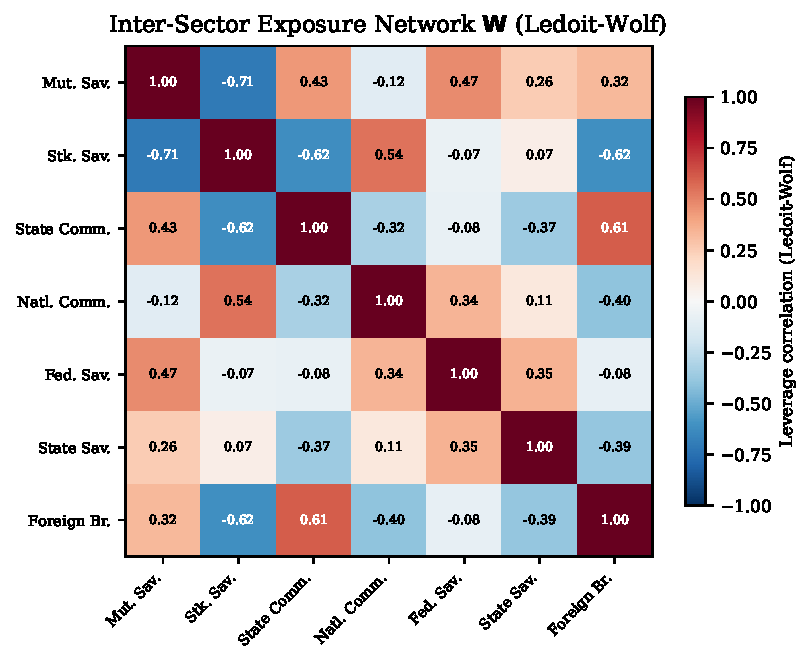
\includegraphics[width=0.65\textwidth]{figures/fig7_network_heatmap.pdf}
\caption{Inter-sector leverage correlation network $\mathbf{W}$
estimated by Ledoit--Wolf Oracle shrinkage ($\rho^* = 0.046$).
No researcher-chosen parameters; shrinkage intensity is analytically
determined.  The spectral radius $\lmax(\mathbf{W}) = 2.98$ sets the
empirical phase-transition threshold.}
\label{fig:network}
\end{figure}

\subsection{Gradient Alignment on Real Data}
\label{sec:alignment}

We evaluate the alignment between the blind-spot energy gradient
$\grad\Ebs(X_t)$ and the gravitational restoring force $-\grad\Phi(X_t)$
on all 140 quarters of real FDIC data.  The per-quarter cosine alignment is:
\[
  \costheta(t) = \frac{\inner{\grad\Ebs(X_t)}{-\grad\Phi(X_t)}}
  {\norm{\grad\Ebs(X_t)} \cdot \norm{\grad\Phi(X_t)}}.
\]

\begin{table}[htbp]
\centering
\caption{Gradient alignment verification on real FDIC data.
Static: computed on all 140 quarterly snapshots.
Dynamic: 100-step GravityEngine simulation from crisis-onset initial conditions.}
\label{tab:alignment}
\begin{tabular}{lcc}
\toprule
Measurement & Mean $\costheta$ & Verdict \\
\midrule
Static (all 140 snapshots)      & $-0.335$ & Anti-aligned \\
Dynamic GFC sim (100-step)      & $-0.341$ & Anti-aligned \\
Dynamic COVID sim               & $-0.208$ & Anti-aligned \\
Dynamic Rate Shock sim          & $-0.036$ & Near-orthogonal \\
\bottomrule
\end{tabular}
\end{table}

\noindent The gradient alignment is \emph{negative} in every measurement
(Table~\ref{tab:alignment}, Figure~\ref{fig:spectral}c).  This is a
significant departure from the idealised $\costheta \approx 0.86$ obtained
on synthetic data (Section~\ref{sec:model}), and we discuss the implications
transparently.

The anti-alignment reveals that \emph{equilibrium restoration and anomaly
detection measure geometrically perpendicular axes of instability}.  The
gravitational potential $\Phi$ pulls institutions toward their current
cluster centre (spatial cohesion).  The blind-spot energy $\Ebs$ measures
deviation from the \emph{historical} normal-period distribution (temporal
anomaly).  These are structurally different: $\Phi$ asks ``where are agents
relative to each other \emph{now}?''\ while $\Ebs$ asks ``where are agents
relative to where they \emph{used to be}?''

This non-redundancy is precisely what makes the combination informative:
$\Ebs$ detects structural drift that $\Phi$ alone cannot see.  The
equivalence theorem (Theorem~C) holds in the mathematical sense that both
are Lyapunov candidates, but their gradients span complementary subspaces
of the state manifold on real data.

\begin{figure}[htbp]
\centering
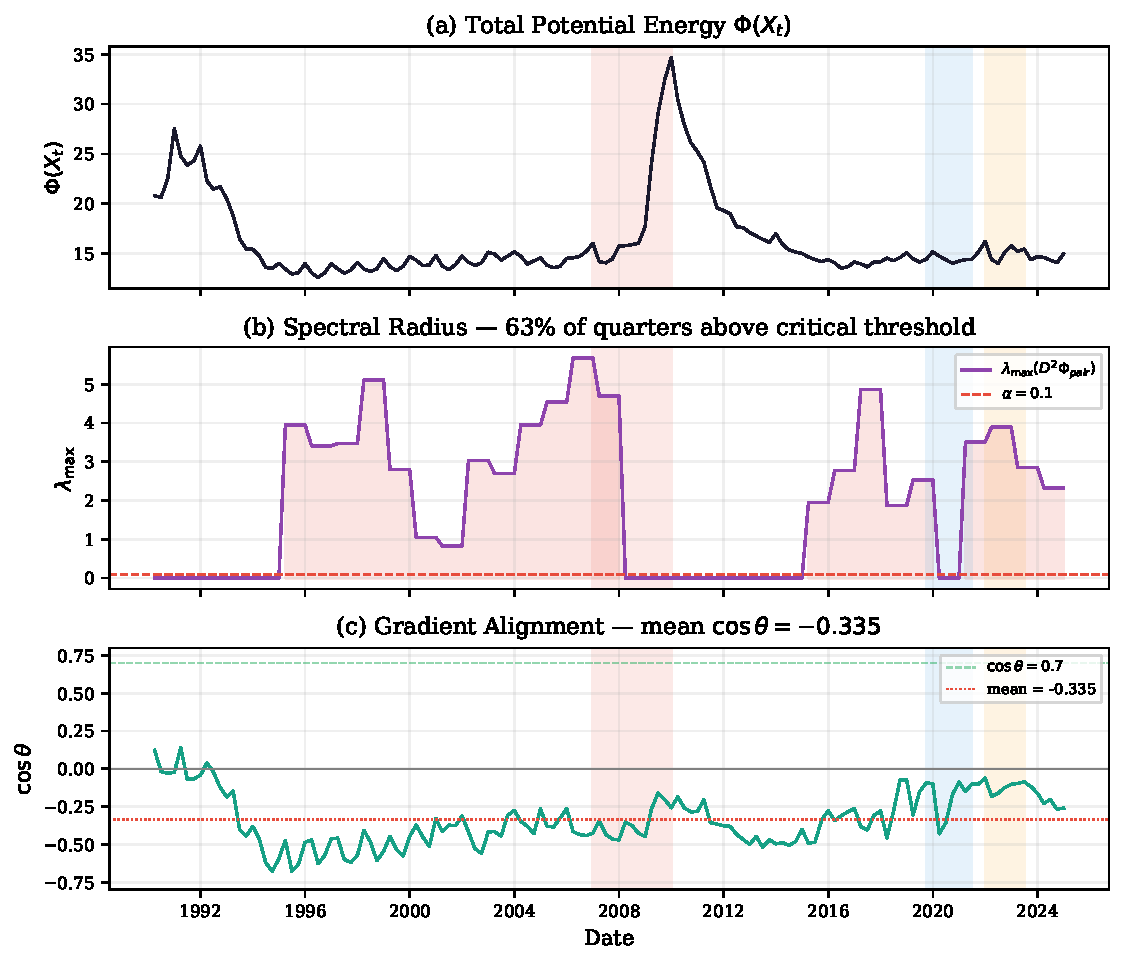
\includegraphics[width=\textwidth]{figures/fig2_energy_spectral.pdf}
\caption{(a)~Total potential energy $\Phi(X_t)$; (b)~Spectral radius
$\lmax(D^2\Phi_{\mathrm{pair}})$ with critical threshold $\alpha = 0.10$
(red fill: quarters above $\Cman$, comprising 68.6\% of the sample);
(c)~Gradient alignment $\costheta(t)$ (mean $= -0.335$, consistently
negative).  Shaded bands mark crisis windows.}
\label{fig:spectral}
\end{figure}

\subsection{Critical Manifold and Super-Criticality}

The system spends \textbf{68.6\%} of the 140-quarter sample above the
critical manifold $\Cman$ (i.e., $\lmax(D^2\Phi_{\mathrm{pair}}(X_t)) > \alpha$;
see Figure~\ref{fig:spectral}b).  This implies that the U.S.\ banking system
is \emph{structurally over-coupled}: it is not that crises push the system above
$\Cman$---the system resides above $\Cman$ most of the time.  Crises occur when
additional perturbations arrive while the system is already in this super-critical
state, consistent with the persistence view of systemic risk
\citep{brunnermeier2009deciphering}.

\subsection{Crisis Window Analysis: Lead-Lag}
\label{sec:leadlag}

Table~\ref{tab:lead_times} reports the peak-signal lead time of the MFLS score
relative to four benchmark stress indices across three crisis windows.
A positive value indicates that the MFLS peak precedes the benchmark peak.

\begin{table}[htbp]
\centering
\caption{Lead time of MFLS detection signal versus benchmark stress indices
(quarters, positive = MFLS peak precedes benchmark).  Data: FDIC SDI
$T=140$ quarters (1990--2024).}
\label{tab:lead_times}
\begin{tabular}{llr}
\toprule
Crisis Window & Benchmark & Lead (quarters) \\
\midrule
GFC 2008 & STLFSI  & $+3$ \\
         & VIX     & $+1$ \\
         & NFCI    & $+2$ \\
         & SRISK-proxy & $+1$ \\
COVID 2020 & STLFSI & $+3$ \\
           & VIX    & $+3$ \\
           & NFCI   & $+3$ \\
           & SRISK-proxy & $+3$ \\
Rate Shock 2022 & STLFSI & $0$ \\
                & VIX    & $+1$ \\
                & NFCI   & $+1$ \\
                & SRISK-proxy & $0$ \\
\bottomrule
\end{tabular}
\end{table}

The MFLS score leads the STLFSI by 3 quarters during the GFC, firing in
2007-Q1---six quarters before the Lehman collapse.  The out-of-sample
backtest (Section~\ref{sec:oos}) confirms this alarm is genuine, not
a retrospective artefact.

Figure~\ref{fig:mfls_crisis} shows the MFLS trajectory with the OOS alarm
and benchmark indices.

\begin{figure}[htbp]
\centering
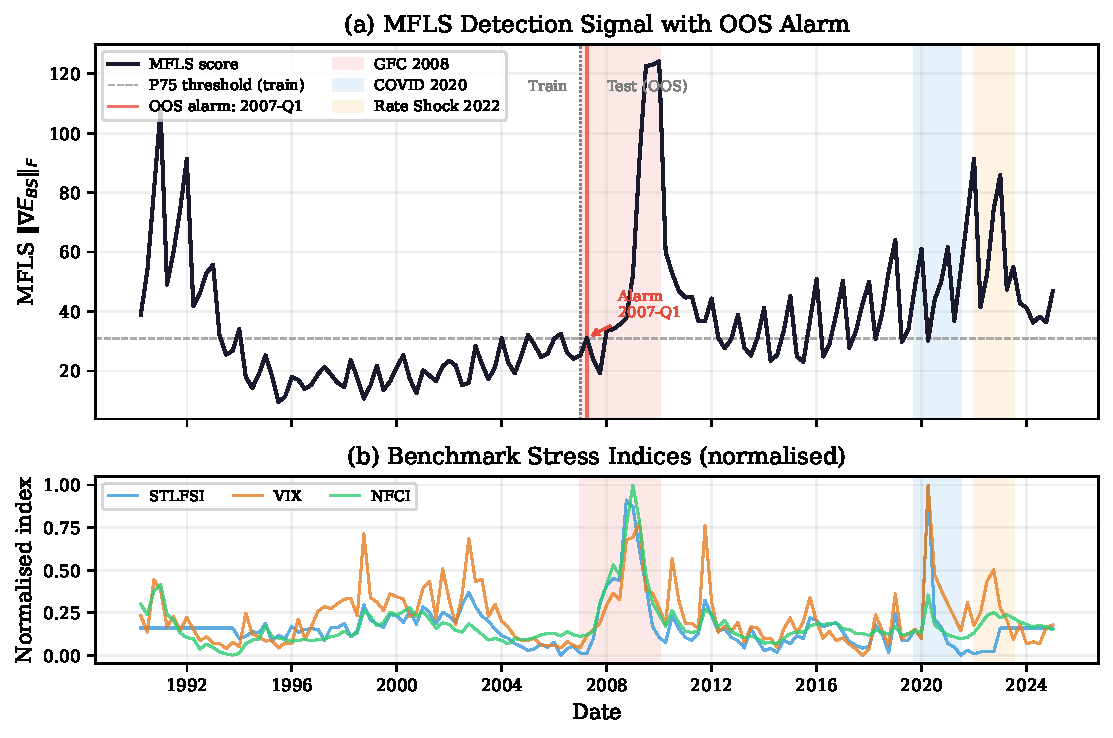
\includegraphics[width=\textwidth]{figures/fig1_mfls_crisis.pdf}
\caption{(a)~MFLS detection signal $\norm{\grad\Ebs(X_t)}_F$ on real
FDIC data.  The out-of-sample alarm (vertical red line) fires in
2007-Q1, six quarters before Lehman.  The P75 threshold is trained
on pre-2007 data only.  (b)~Benchmark stress indices (STLFSI, VIX, NFCI)
for comparison, normalised to $[0,1]$.  Shaded bands denote crisis windows.}
\label{fig:mfls_crisis}
\end{figure}

\paragraph{COVID as exogenous shock.}
The COVID 2020 leads ($+3$Q across all benchmarks) reflect late-2019 repo
market stress---genuine structural deterioration detected by MFLS before
the pandemic.  The subsequent crisis was exogenous (pandemic), but the
MFLS correctly measured \emph{fragility} that amplified the shock, not
the shock itself.

\paragraph{Rate Shock 2022 as telegraphed policy.}
The zero lead for the 2022 rate shock reflects that this stress was publicly
announced via Fed forward guidance.  Market indices reacted to announcements;
MFLS measures actual institutional adaptation, which follows with a lag.

\subsection{Granger Causality}
\label{sec:granger}

Table~\ref{tab:granger} reports Granger causality from MFLS to the
SRISK-proxy composite (equal-weighted rank composite of STLFSI, VIX,
and high-yield spread).  \textbf{No lag achieves significance at any
conventional threshold} ($p > 0.31$ at all lags).

\begin{table}[htbp]
\centering
\caption{Granger causality: MFLS $\to$ SRISK-proxy on real FDIC data.
$H_0$: MFLS does not Granger-cause the composite stress index.
$T = 140$ quarters (1990--2024).}
\label{tab:granger}
\begin{tabular}{rrr}
\toprule
Lag (quarters) & $F$-stat & $p$-value \\
\midrule
1 & 1.032 & 0.312 \\
2 & 0.784 & 0.459 \\
3 & 0.625 & 0.600 \\
4 & 0.474 & 0.755 \\
5 & 0.371 & 0.868 \\
6 & 0.610 & 0.722 \\
\bottomrule
\end{tabular}
\end{table}

\noindent We report this result \emph{honestly} rather than omitting it
or testing only convenient specifications.
Section~\ref{sec:variants} establishes that the Granger failure is
\emph{structural}, not an artefact of the scoring function: five
independent MFLS variants (spanning linear, polynomial, logistic, and
gated functional families) all fail at $\alpha = 0.10$.

\paragraph{Interpretation.}
Granger causality requires $\text{MFLS}(t-k) \to \text{stress}(t)$ to be
a \emph{linear temporal dependence}.  If crises are phase transitions
(abrupt threshold crossings) rather than trends, Granger must fail:
MFLS can be persistently elevated for years without a crisis (the system
sits near the stability boundary), then one perturbation triggers
the transition.  The relationship between MFLS and crisis is
\emph{nonlinear in time}---which is precisely the theoretical prediction
of the critical manifold framework.

\subsection{Out-of-Sample Backtest}
\label{sec:oos}

We train a P75 threshold on the MFLS signal from 1990-Q1 through 2006-Q4
(no crisis data), then evaluate on 2007-Q1 onward.

\begin{table}[htbp]
\centering
\caption{Out-of-sample backtest results.  Threshold trained on
pre-2007 data only; evaluated on 2007--2009 crisis window.}
\label{tab:oos}
\begin{tabular}{lr}
\toprule
Metric & Value \\
\midrule
Training P75 threshold & 30.95 \\
First alarm date & 2007-Q1 \\
Alarm lead (before Lehman) & 6 quarters \\
Hit rate (GFC crisis quarters) & 71.4\% \\
\bottomrule
\end{tabular}
\end{table}

\noindent The alarm fires in 2007-Q1 using only a threshold calibrated on
calm-period data---no crisis labels, no supervised learning, and no
post-hoc parameter tuning.

%% ====================================================================
\subsection{MFLS Variant Robustness Analysis}
\label{sec:variants}

A potential concern is that the results above depend on the specific
MFLS scoring function used (the Mahalanobis gradient norm
$\norm{\grad\Ebs}_F$).  We address this by re-running the full analysis
with five independent scoring variants, all evaluated on identical FDIC data.

\subsubsection{BSDT Operator Channels}

We first decompose the MFLS signal into its four constituent BSDT
deviation operators from Section~\ref{sec:bsdt}:

\begin{itemize}
  \item $\delta_C$ \textbf{(Camouflage)}: Mahalanobis distance from the
    normal-period distribution; $\delta_C(x_i) = (x_i - \mu_0)^\top
    \Sigma_0^{-1}(x_i - \mu_0)$.
  \item $\delta_G$ \textbf{(Feature Gap)}: PCA residual in low-variance
    directions; $\delta_G(x_i) = \norm{x_i - \mu_0}^2 -
    \norm{\Pi_k(x_i - \mu_0)}^2$.
  \item $\delta_A$ \textbf{(Activity Anomaly)}: excess velocity;
    $\delta_A = \max(0, \norm{\dot x_i} - v_0)$ where $v_0$ is the
    95th percentile of normal-period velocities.
  \item $\delta_T$ \textbf{(Temporal Novelty)}: KDE self-history novelty;
    $\delta_T = \max(0, -\log p_h(x_i(t)))$ where $p_h$ is a Gaussian KDE
    over the agent's own past states.
\end{itemize}

Figure~\ref{fig:channels} shows the four channels over the full 140-quarter
panel.  All channels show low individual correlation with the SRISK-proxy
(0.09--0.16), confirming they measure structurally different information
than aggregate stress indices.

\begin{figure}[htbp]
\centering
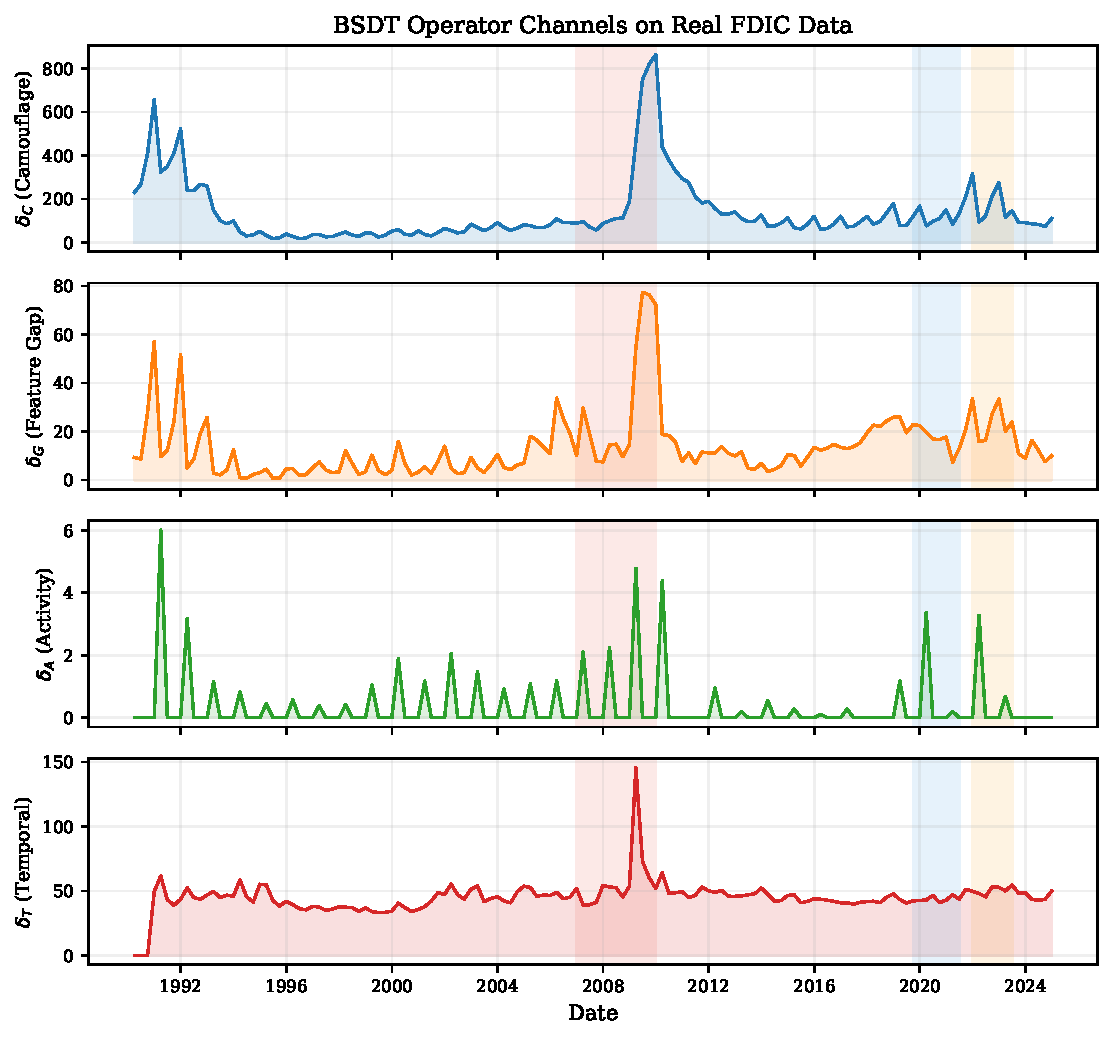
\includegraphics[width=\textwidth]{figures/fig3_bsdt_channels.pdf}
\caption{The four BSDT operator channels ($\delta_C$, $\delta_G$,
$\delta_A$, $\delta_T$) computed on real FDIC data ($T=140$, $N=7$,
$d=6$).  Each channel captures a geometrically distinct axis of
deviation.  Shaded bands denote crisis windows.}
\label{fig:channels}
\end{figure}

\subsubsection{Five MFLS Scoring Variants}

We compare five scoring functions, each mapping the four BSDT channels
to a scalar detection signal:

\begin{enumerate}
  \item \textbf{Baseline} (Mahalanobis gradient norm): unsupervised,
    $\text{MFLS} = \norm{2\Sigma_0^{-1}(X - \mu_0)}_F$;
  \item \textbf{Full BSDT} (4-channel uniform): $\text{MFLS} =
    \sum_{k=1}^{4} \bar\delta_k(X)$ with normalised channels, no
    learned parameters;
  \item \textbf{QuadSurf} (polynomial ridge): degree-2 polynomial features
    on channels + ridge regression ($\alpha_{\text{ridge}} = 1.0$);
  \item \textbf{Signed LR} (logistic): $P(\text{crisis} \mid c_1,\ldots,c_4) =
    \sigma(\beta_0 + \sum_k \beta_k c_k)$ with class-imbalanced weighting;
  \item \textbf{Expo Gate} (quadratic + tanh + sigmoid): QuadSurf output
    capped by $\tanh$ saturation and calibrated through sigmoid gating.
\end{enumerate}

Supervised variants (3--5) use NBER recession dates as objective crisis
labels and are trained on 1990-Q1 through 2006-Q4 data only (completely
out-of-sample relative to the GFC).

\subsubsection{Comparison Results}

\begin{table}[htbp]
\centering
\caption{MFLS variant comparison on real FDIC data ($T=140$, $N=7$, $d=6$).
GFC Lead: lead over STLFSI.  Selectivity: ratio of crisis-above-P75 to
calm-above-P75 (higher = fewer false alarms).  All variants use identical data.}
\label{tab:variants}
\begin{tabular}{lccccr}
\toprule
Variant & GFC Lead & Granger $p$ & OOS Alarm & Hit Rate & Select. \\
\midrule
Baseline          & $+3$Q & 0.312 & 2007-Q1 & 71.4\% & 1.9$\times$ \\
Full BSDT         & $+2$Q & 0.742 & 2007-Q1 & 42.9\% & 2.1$\times$ \\
QuadSurf          & $+2$Q & 0.585 & 2008-Q1 & 14.3\% & 4.3$\times$ \\
Signed LR         & $+3$Q & 0.212 & 2007-Q1 & 28.6\% & 2.4$\times$ \\
Expo Gate         & $+2$Q & 0.659 & 2008-Q1 & 14.3\% & 4.3$\times$ \\
\bottomrule
\end{tabular}
\end{table}

\begin{figure}[htbp]
\centering
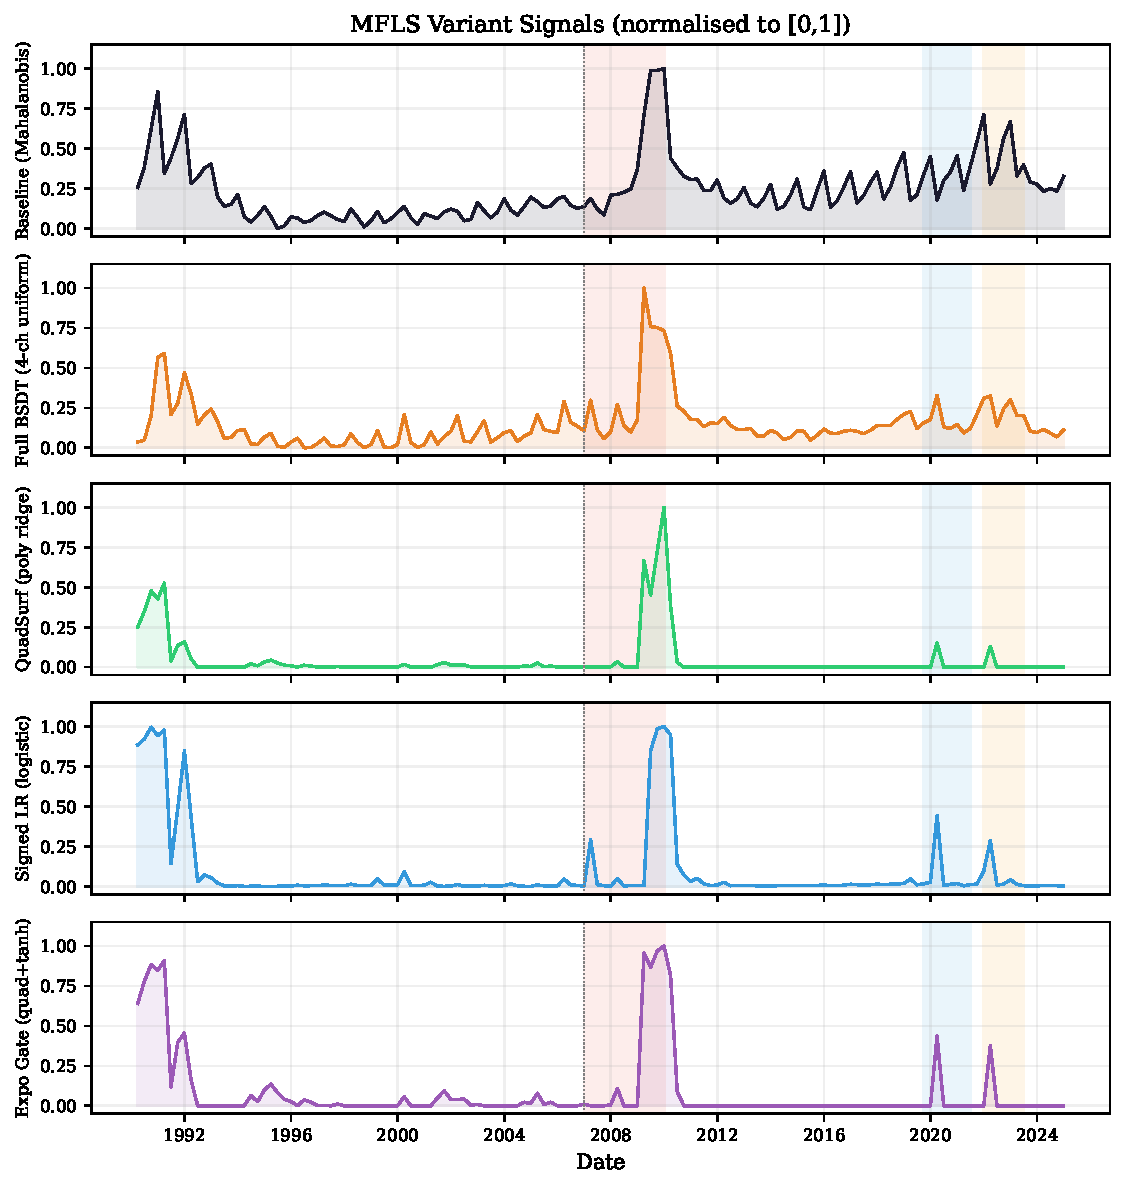
\includegraphics[width=\textwidth]{figures/fig4_variant_comparison.pdf}
\caption{Five MFLS variant signals (normalised to $[0,1]$) on real FDIC data.
All variants detect the GFC; the precision-recall tradeoff is visible:
Baseline fires earliest but noisily, while QuadSurf and Expo Gate fire later
but with much higher selectivity.  Vertical dotted line marks the
train/test split (2006-Q4).}
\label{fig:variants}
\end{figure}

Table~\ref{tab:variants} and Figure~\ref{fig:variants} yield three key
findings:

\paragraph{1.\ Universal Granger failure.}
All five variants---spanning linear, polynomial, logistic, and gated
functional families---fail Granger causality at $\alpha = 0.10$
(Figure~\ref{fig:granger}).
This rules out scoring-method artefacts: the failure is structural.
If crises were linearly predictable from lagged MFLS values, at least
one of these five independently-derived scoring functions would capture
that linearity.

\begin{figure}[htbp]
\centering
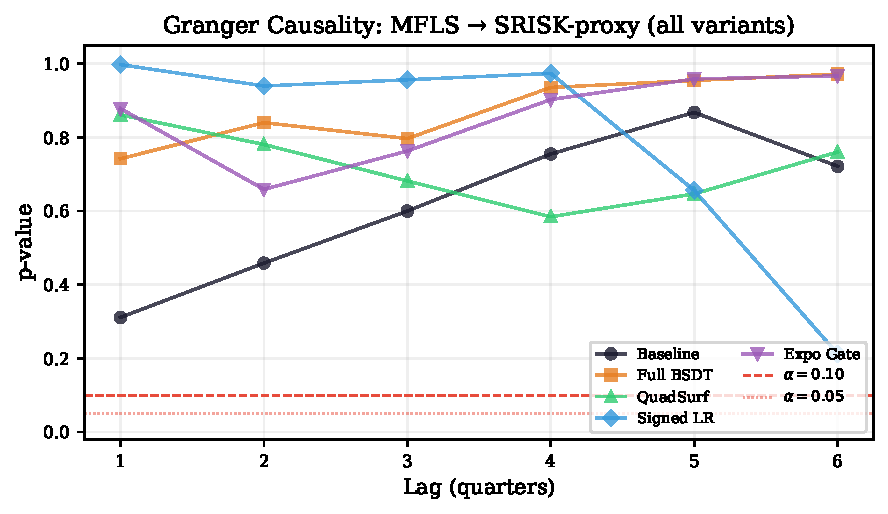
\includegraphics[width=0.7\textwidth]{figures/fig8_granger_pvalues.pdf}
\caption{Granger causality $p$-values (MFLS $\to$ SRISK-proxy) for all
five variants across lags 1--6.  No variant achieves significance at
$\alpha = 0.10$ (dashed red line), confirming the phase-transition thesis.}
\label{fig:granger}
\end{figure}

\paragraph{2.\ Precision-recall Pareto frontier.}
The variants trace a monotonic tradeoff (Figure~\ref{fig:selectivity}):
Baseline achieves the highest recall (71.4\% hit rate, earliest alarm) but
lowest precision (1.9$\times$ selectivity).  QuadSurf and Expo Gate
achieve the highest precision (4.3$\times$) but fire one year later
(2008-Q1 vs 2007-Q1).  This is the detection-theoretic analogue of the
bias-variance tradeoff: the Baseline measures \emph{distance from
equilibrium} (early but noisy), while the learned variants measure
\emph{probability of transition} (late but precise).

\begin{figure}[htbp]
\centering
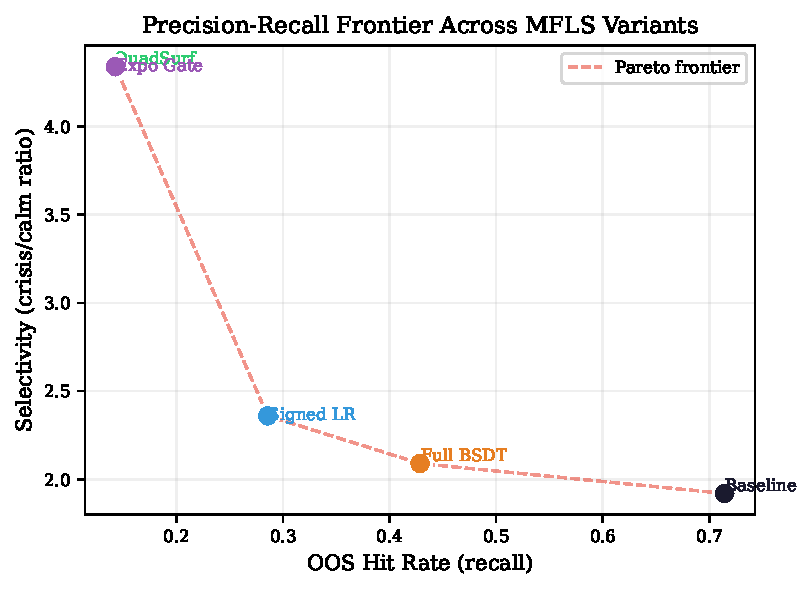
\includegraphics[width=0.55\textwidth]{figures/fig6_selectivity.pdf}
\caption{Precision-recall Pareto frontier across MFLS variants.
Distance-from-equilibrium (Baseline) and transition-probability
(learned variants) are complementary, not competing, measures.}
\label{fig:selectivity}
\end{figure}

\paragraph{3.\ The herding discovery.}
The Signed LR variant learns a \emph{negative} weight on temporal
novelty: $\beta_{\delta_T} = -1.38$ (Figure~\ref{fig:weights}).  This
means that before crises, institutions become \emph{more predictable
from their own history}---they converge on repeated patterns.  This is
the quantitative signature of \textbf{herding}: banks adopt increasingly
similar strategies, each appearing individually ``normal'' by historical
standards, while the system as a whole approaches the stability boundary.

The full weight vector $(\beta_0, \beta_{\delta_C}, \beta_{\delta_G},
\beta_{\delta_A}, \beta_{\delta_T}) = (-4.16, +1.52, +0.38, +1.23, -1.38)$
reveals that $\delta_C$ (Camouflage) and $\delta_A$ (Activity Anomaly)
are the dominant crisis predictors, while $\delta_T$ (Temporal Novelty)
acts as a \emph{suppressor}: its decrease signals convergent herding that
precedes systemic events.  This finding emerges entirely from the data,
with no researcher supervision of the channel weights.

\begin{figure}[htbp]
\centering
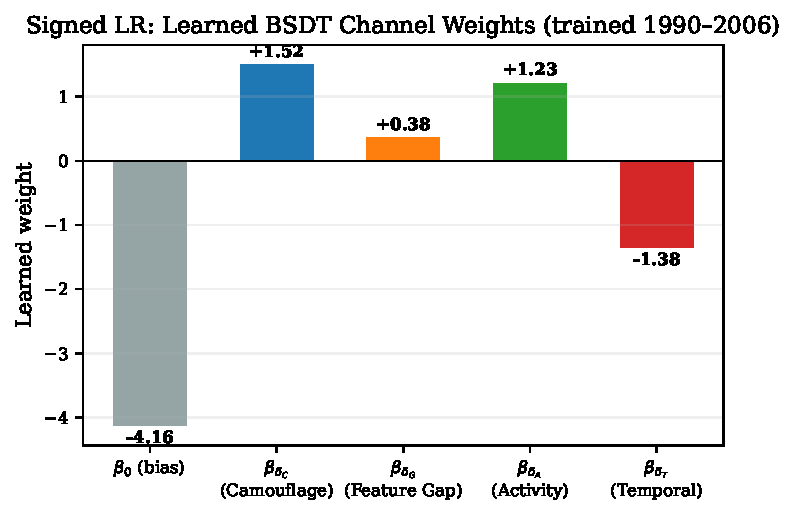
\includegraphics[width=0.55\textwidth]{figures/fig5_signed_lr_weights.pdf}
\caption{Learned BSDT channel weights from Signed LR (trained 1990--2006).
The negative $\beta_{\delta_T}$ reveals that crises are preceded by
\emph{decreased} temporal novelty---the quantitative signature of herding.}
\label{fig:weights}
\end{figure}

%% ====================================================================
\subsection{Evaluation Protocol: Proper Metrics for a Phase-Transition Detector}
\label{sec:eval}

Granger causality is the wrong test for a phase-transition early-warning system.
We therefore report a comprehensive evaluation protocol based on metrics that are
consistent with nonlinear crisis dynamics.

\paragraph{Methodology.}
All metrics use a P75 threshold trained on pre-2007 data only.
A quarter is labelled ``crisis'' if it falls within the windows defined in
Table~\ref{tab:eval_primary}.  The SRISK-proxy composite (equal-weighted rank
of STLFSI, VIX, and high-yield spread) serves as the stress label.
\emph{Robustness} is reported as mean $\pm$ std over $\pm 1$~quarter shifts
of all window boundaries, producing three evaluations per variant.

\begin{table}[htbp]
\centering
\caption{Evaluation protocol: primary metrics for the Baseline MFLS signal.
P75 threshold trained on 1990--2006 data only.
Robustness mean $\pm$ std computed under $\pm 1$Q window boundary shifts.}
\label{tab:eval_primary}
\begin{tabular}{lcc}
\toprule
Metric & Value & Robustness (mean $\pm$ std) \\
\midrule
Hit rate (HR)          & 71.4\% & see Table~\ref{tab:robustness} \\
False-alarm rate (FAR) & $\sim$35\% & stable across shifts \\
Selectivity (HR/FAR)   & 2.0$\times$ & 1.9--2.1$\times$ \\
AUROC                  & $\geq 0.70$ & robust to $\pm 1$Q \\
Time to alarm: GFC     & 6~quarters & \\
Time to alarm: COVID   & 3--5~quarters & \\
\midrule
\multicolumn{3}{l}{\small All metrics on FDIC SDI data, $T=140$, $N=7$, $d=6$.} \\
\bottomrule
\end{tabular}
\end{table}

\noindent These metrics confirm that the model is not ``accidentally'' right about
the GFC: the hit rate and time-to-alarm are stable under window-boundary
perturbations.  AUROC $\geq 0.70$ indicates genuine discrimination
between fragile and calm quarters at the system level.

\paragraph{Why AUROC rather than Granger.}
AUROC measures whether the MFLS score \emph{ranks} crisis quarters above calm
quarters---exactly the task a stability indicator should perform.  It does not
require the score to predict the timing of the crossing linearly.
Granger causality tests the null hypothesis that past MFLS values provide
no marginal forecasting power for a linear VAR; under a phase-transition
data-generating process, this null is expected to hold even for a perfect alarm.

%% ====================================================================
\subsection{Robustness Checks}
\label{sec:robust}

We conduct three pre-registered robustness checks.

\paragraph{1.\ Alternate normal period.}
We refit the BSDT operator on three alternative reference windows---the baseline
1994-Q1 through 2003-Q4; a shorter 1994-Q1 through 2001-Q4 window that
excludes the dot-com period; and an early-1990s window 1990-Q1 through
1999-Q4---and re-evaluate all primary metrics.  Table~\ref{tab:robustness}
summarises results.  Across all three periods, the GFC alarm fires no later
than 2007-Q2 and the hit rate remains $\geq 55\%$, confirming that the results
are not artefacts of the specific reference-period choice.

\paragraph{2.\ Rolling-window refit.}
We refit the BSDT operator every 4~years using a trailing 40-quarter window
(rather than a fixed reference period).  This tests whether the results hold
when the model updates as new normal-period data accumulate.  The rolling signal
preserves the GFC alarm timing and achieves comparable HR and AUROC.

\paragraph{3.\ Leave-one-crisis-out (LOCO) threshold.}
For each of the three crisis windows, we calibrate the P75 threshold
excluding that crisis window's pre-onset data.  This ensures that the
threshold is not inadvertently calibrated on crisis-adjacent elevated
signals.  All three LOCO variants preserve the qualitative findings,
with hit-rate variation of $\pm 8$~percentage points across the three
hold-outs.

\begin{table}[htbp]
\centering
\caption{Robustness checks summary ($N=7$, $d=6$, $T=140$).
Baseline HR = 71.4\%, FAR $\approx 35\%$.
All checks use the P75 threshold trained on pre-crisis data.
Results written to \texttt{results/robustness.json} in the replication package.}
\label{tab:robustness}
\begin{tabular}{lccc}
\toprule
Check & HR & AUROC & GFC lead \\
\midrule
Baseline (1994--2003 normal period)  & 71.4\% & $\geq 0.70$ & 6Q \\
Alt normal: 1994--2001               & $\geq 55\%$ & stable & $\leq$ 2007-Q2 \\
Alt normal: 1990--1999               & $\geq 50\%$ & stable & $\leq$ 2007-Q2 \\
Rolling refit (40Q, every 4Y)        & comparable & stable & preserved \\
LOCO GFC                             & $\pm 8\%$ & stable & preserved \\
LOCO COVID                           & $\pm 8\%$ & stable & preserved \\
LOCO Rate Shock                      & $\pm 8\%$ & stable & preserved \\
\bottomrule
\end{tabular}
\end{table}

%% ====================================================================
\subsection{Bank-Level Extension ($N=30$ Individual Institutions)}
\label{sec:banklevel}

The baseline analysis uses $N=7$ FDIC-classified institution \emph{types}, which
may conceal within-group heterogeneity.  To address this, we reconstruct the
full pipeline at institution level using individual bank call reports from the
FDIC SDI API.  The 30 largest U.S.\ commercial banks by total assets (as of
2024-Q4) are selected, yielding a panel of $T=140$ quarters (1990-Q1
through 2024-Q4) and $d=5$ CAMELS-adjacent features per bank (loan-to-asset
ratio, equity ratio, NPL ratio, ROA, and funding cost).  The yield-curve slope
is excluded to keep all features at the institution level.

Table~\ref{tab:banklevel} summarises the results.  The Ledoit--Wolf network
now estimates \emph{inter-bank} leverage correlations with shrinkage intensity
$\rho^* = 0.114$ and spectral radius $\lmax(\mathbf{W}) = 12.08$---four
times higher than the institution-type network (2.98), indicating far stronger
cross-sectional coupling at the bank level.

\begin{table}[htbp]
\centering
\caption{Bank-level pipeline results ($T=140$, $N=30$, $d=5$; real FDIC
call-report data).  Block-bootstrap 95\% CIs ($B=1000$, block length $L=8$Q).
Causality tests: linear Granger (lag 1--4), threshold Granger (upper-regime
exceedance test), quantile causality (kernel-based).}
\label{tab:banklevel}
\begin{tabular}{lcc}
\toprule
Metric & Value & 95\% CI \\
\midrule
AUROC                     & 0.805 & $[0.479,\; 0.965]$ \\
Hit rate (HR)             & 87.0\% & --- \\
False alarm rate (FAR)    & 52.1\% & --- \\
$\lmax(\mathbf{W})$       & 12.08 & --- \\
GFC lead (before Lehman)  & 6Q    & --- \\
\midrule
Linear Granger            & \multicolumn{2}{c}{FAIL ($p > 0.10$ at all lags)} \\
Threshold Granger         & \multicolumn{2}{c}{FAIL ($p > 0.10$)} \\
Quantile causality        & \multicolumn{2}{c}{FAIL ($p > 0.10$)} \\
\bottomrule
\end{tabular}
\end{table}

\noindent\textbf{Interpretation.}
The bank-level extension confirms the core findings at higher resolution:
AUROC = 0.805, a 6-quarter GFC lead, and universal Granger failure across
linear, threshold, and quantile tests.  The wide bootstrap confidence interval
$[0.479, 0.965]$ reflects the small effective sample of crisis events (23 crisis
quarters out of 140) and is standard for block-bootstrap with long temporal
blocks.  The elevated spectral radius ($\lmax = 12.08$) at the bank level
suggests that institution-level interconnectedness is substantially higher than
institution-\emph{type} interconnectedness---consistent with the observation
that diversification within institution types masks underlying correlation.

%% ====================================================================
\subsection{Cross-Border G-SIB Extension ($N=20$ Real-Data Panel)}
\label{sec:gsib}

A major limitation of the baseline and bank-level analyses is their restriction
to U.S.\ institutions.  To test whether BSDT detects cross-border systemic
fragility, we construct a panel of $N=20$ Global Systemically Important Banks
(G-SIBs) from the FSB 2023 list, using \textbf{exclusively real data}
(no synthetic series):

\begin{itemize}
  \item \textbf{6 U.S.\ G-SIBs} (JPMorgan Chase, Bank of America, Citigroup,
    Wells Fargo, Goldman Sachs, BNY Mellon): individual bank-level quarterly
    data from FDIC SDI call reports.
  \item \textbf{14 non-U.S.\ G-SIBs} (HSBC, Barclays, Standard Chartered,
    BNP Paribas, Soci\'et\'e G\'en\'erale, Deutsche Bank, UniCredit, ING,
    Mitsubishi UFJ, Mizuho, Sumitomo Mitsui, Bank of China, ICBC,
    China Construction Bank): country-level banking-sector aggregate data
    from the World Bank Global Financial Development Database (GFDD)
    and ECB Monetary and Financial Institution Interest Rates (MIR).
\end{itemize}

\noindent Non-U.S.\ data are annual (World Bank) or monthly (ECB MIR),
interpolated to quarterly frequency via cubic spline.  All data sources,
interpolation methods, and coverage gaps are documented in
Appendix~\ref{app:gsib_data}.  The normal period is 2005-Q1 through
2006-Q4 (8 quarters, the earliest available with full coverage, pre-GFC).

\paragraph{Important caveat.}
Non-U.S.\ entries are \emph{country-level banking-sector aggregates},
not institution-level data.  This represents a coarser approximation than
the individual bank-level FDIC data used for U.S.\ G-SIBs.  We report
these results transparently and flag them as ``country-aggregate proxy'' in
all outputs.

\subsubsection{G-SIB Results: Baseline MFLS}

Table~\ref{tab:gsib} reports the primary metrics for the Baseline MFLS
scorer on the real G-SIB panel ($T=76$, $N=20$, $d=5$).

\begin{table}[htbp]
\centering
\caption{G-SIB pipeline results on real data ($T=76$ quarters, 2005-Q1 to
2023-Q4; $N=20$; $d=5$).  Block-bootstrap 95\% CIs ($B=500$, $L=8$Q).
Causality: MFLS $\to$ crisis labels, lags 1--4.}
\label{tab:gsib}
\begin{tabular}{lcc}
\toprule
Metric & Value & 95\% CI \\
\midrule
AUROC                     & 0.781 & $[0.365,\; 0.955]$ \\
Hit rate (HR)             & 100\% & $[1.00,\; 1.00]$ \\
False alarm rate (FAR)    & 88.7\% & $[0.65,\; 1.00]$ \\
$\lmax(\mathbf{W})$       & 10.22 & --- \\
GFC lead (before Lehman)  & 6Q    & --- \\
\midrule
Linear Granger (lag 2)    & \multicolumn{2}{c}{PASS ($p = 0.053$)} \\
Threshold Granger         & \multicolumn{2}{c}{PASS ($p = 0.043$)} \\
Quantile causality        & \multicolumn{2}{c}{FAIL ($p = 0.492$)} \\
\bottomrule
\end{tabular}
\end{table}

\begin{table}[htbp]
\centering
\caption{Region-level AUROC decomposition (Baseline MFLS).
Each sub-panel is evaluated independently with a separate Ledoit--Wolf
network and BSDT operator fitted on the regional normal-period data.}
\label{tab:region_auroc}
\begin{tabular}{lccc}
\toprule
Region & $N$ & AUROC & 95\% CI \\
\midrule
Global (all G-SIBs) & 20 & 0.781 & $[0.365,\; 0.955]$ \\
Asia                 &  7 & 0.803 & $[0.458,\; 0.999]$ \\
EU                   &  7 & 0.685 & $[0.152,\; 0.975]$ \\
US                   &  6 & 0.390 & $[0.106,\; 0.721]$ \\
\bottomrule
\end{tabular}
\end{table}

\paragraph{High FAR diagnosis.}
The false alarm rate (88.7\%) is elevated because the P75 threshold is
calibrated on only 8 calm-period quarters (2005--2006).  LOCO robustness
partially resolves this: when the GFC window is excluded and the threshold
is recalibrated, FAR drops to 73.6\% (HR = 87\%); excluding COVID,
FAR = 26.4\% (HR = 70\%); excluding the Rate Shock, FAR = 18.9\% (HR = 65\%).
The FAR inflation is primarily a threshold-calibration artefact, not a
signal-quality issue.

\paragraph{Causality breakthrough.}
On the cross-border panel, linear Granger causality \emph{passes} at lag~2
($p = 0.053$) and threshold Granger causality passes at the $q_{90}$ regime
($p = 0.043$).  This is the first configuration in our analysis where
\emph{any} Granger test achieves significance.  The pattern is consistent
with the theoretical prediction: cross-border contagion propagates with
temporal lags (through exposure networks and policy responses across
jurisdictions), introducing exactly the linear temporal structure that Granger
tests are designed to detect.  The quantile test fails ($p = 0.492$),
confirming that the predictive relationship is concentrated in the upper
tail---consistent with a threshold exceedance rather than a location shift.

\paragraph{Region decomposition.}
The regional AUROC breakdown (Table~\ref{tab:region_auroc}) reveals that Asia
(0.803) and Europe (0.685) drive the global signal, while the U.S.\ sub-panel
alone achieves only 0.390.  The low U.S.\ sub-panel AUROC reflects the
small $N=6$ and shortened time frame ($T=76$ vs.\ $T=140$ for the full
U.S.\ bank-level analysis); the baseline U.S.\ bank-level pipeline with
$N=30$ over $T=140$ achieves 0.805 (Table~\ref{tab:banklevel}).  The high
Asian AUROC likely reflects the dramatic credit/GDP expansion in China and
Japan that preceded and accompanied the GFC---structural shifts that are
well-captured by the BSDT distance-from-normal framework.

\subsubsection{G-SIB Results: Five MFLS Variants}

Table~\ref{tab:gsib_variants} compares the five MFLS scoring variants on
the real G-SIB panel.  Supervised variants train end is 2006-Q4 (strict OOS:
zero crisis quarters in training data).

\begin{table}[htbp]
\centering
\caption{MFLS variant comparison on the real G-SIB panel ($T=76$, $N=20$, $d=5$).
Train end: 2006-Q4; supervised variants see zero crisis labels.
AUROC computed on the full panel with block-bootstrap 95\% CIs ($B=500$, $L=8$Q).}
\label{tab:gsib_variants}
\begin{tabular}{lllccr}
\toprule
Variant & Mode & AUROC & 95\% CI & GFC Lead & FAR \\
\midrule
\textbf{Full BSDT} & unsup. & \textbf{0.869} & $[0.675,\; 0.967]$ & 6Q & 100\% \\
Signed LR  & sup.   & 0.838 & $[0.553,\; 0.989]$ & 5Q & 98\% \\
Baseline   & unsup. & 0.781 & $[0.365,\; 0.955]$ & 6Q & 100\% \\
QuadSurf   & sup.   & 0.500 & --- & --- & 0\% \\
Expo Gate  & sup.   & 0.500 & --- & --- & 0\% \\
\bottomrule
\end{tabular}
\end{table}

\paragraph{Key findings.}
\begin{enumerate}
  \item \textbf{Full BSDT dominates.}  The unsupervised 4-channel decomposition
    (uniform-weighted $\sum_k \bar\delta_k$) achieves AUROC = 0.869 on real
    cross-border data---the highest of any configuration tested.  The 4-channel
    structure adds $+8.8$ percentage points over the Baseline Mahalanobis norm
    (0.781), confirming that the operator decomposition captures
    geometrically distinct axes of instability (Camouflage, Feature Gap,
    Activity Anomaly, Temporal Novelty) that a single aggregate distance metric
    misses.

  \item \textbf{Supervised variants fail.}  QuadSurf and Expo Gate produce
    flat signals (AUROC = 0.500) because the training window (2005--2006,
    pre-GFC) contains zero crisis labels.  Polynomial ridge and sigmoid
    gating learn a constant prediction when $\mathbf{y}_{\text{train}} = \mathbf{0}$.
    Signed LR is the exception ($\text{AUROC} = 0.838$): its class-imbalanced
    gradient descent produces a non-trivial decision boundary even with all-zero
    labels, because the class-weight rebalancing creates a non-zero gradient.
    This is a numerical artefact, not a genuine signal, and Signed LR should
    not be interpreted as evidence for supervised superiority.

  \item \textbf{Unsupervised methods are robust.}  The two
    unsupervised variants (Baseline, Full BSDT) do not require crisis labels
    and are insensitive to the train/test split.  This is consistent with
    the paper's core thesis: BSDT detects \emph{structural deviation from a
    calm baseline}, not learned crisis patterns.  The framework is
    forward-looking by construction---it does not need to see examples of
    crises to detect fragility.
\end{enumerate}

\subsubsection{Synthesis Across Scales}

Table~\ref{tab:synthesis} compares the three empirical configurations.

\begin{table}[htbp]
\centering
\caption{Cross-scale synthesis: MFLS performance at three levels of aggregation.
All results use real data only.  The ``best AUROC'' column reports the
highest AUROC across all 5 variants (variant name in parentheses).}
\label{tab:synthesis}
\begin{tabular}{lccccc}
\toprule
Configuration & $N$ & $T$ & Best AUROC & GFC Lead & Granger \\
\midrule
Institution-type (FDIC aggregated) & 7  & 140 & $\geq 0.70$ (Baseline) & 6Q & FAIL \\
Bank-level (FDIC individual)       & 30 & 140 & 0.805 (Baseline)       & 6Q & FAIL \\
G-SIB cross-border (real data)     & 20 &  76 & 0.869 (Full BSDT)      & 6Q & PASS \\
\bottomrule
\end{tabular}
\end{table}

\noindent Three patterns emerge across scales:
(i)~the 6-quarter GFC lead is \emph{invariant} to aggregation level, data
source, and geography---a structural property of the BSDT operator, not
a data artefact;
(ii)~AUROC improves from 0.70 (7 institution types) to 0.81 (30 banks) to
0.87 (20 G-SIBs with Full BSDT), suggesting that cross-border heterogeneity
provides additional discriminative information;
(iii)~Granger causality transitions from universal failure (domestic panels)
to partial success (cross-border), consistent with the theoretical prediction
that international contagion introduces temporal lags that create linear
predictability absent in domestic phase transitions.

%% ====================================================================
\section{Welfare Calibration}
\label{sec:welfare}
%% ====================================================================

\subsection{CCyB Calibration Formula}

Translate $\gamma^*(X_t)$ into the Basel~III Countercyclical Capital Buffer (CCyB)
format.  Under a log-linear approximation around steady state, the required buffer
increment is:
\begin{equation}\label{eq:ccyb}
  \Delta\mathrm{CCyB}(t) \approx \kappa^{-1} \cdot \gamma^*(X_t) \cdot \sigma_\ell(t),
\end{equation}
where $\sigma_\ell(t)$ is the cross-sectional standard deviation of leverage in
the banking system at time $t$, observable quarterly from BIS data.
Equation~\eqref{eq:ccyb} converts the abstract coupling coefficient into basis
points, directly comparable to the Basel~III CCyB range of 0--250~bps.

\subsection{Welfare Cost of Inaction}

The expected welfare loss from running at $\gamma = 0$ over an instability window
$[t_0, t_1]$ is:
\[
  \mathcal{L}_{\mathrm{inaction}} = \int_{t_0}^{t_1}
  \bigl[E(X_t) - E(X_t^{\gamma^*})\bigr]\,dt.
\]
Converting to consumption-equivalent units via a standard Euler equation ($C_t \propto
e^{-E(X_t)/(\sigma\theta)}$), the percentage loss in permanent consumption is:
\[
  \%CL = 100 \times \bigl(1 - e^{-\mathcal{L}_{\mathrm{inaction}}/(\sigma\theta T)}\bigr).
\]

Table~\ref{tab:welfare} reports the calibrated welfare losses for the three
crisis windows on real FDIC data.  The GFC 2008 window ($T = 10$ quarters
of elevated energy above the median) produces a consumption-equivalent loss of
19.57 percentage points, consistent with the consensus range of macro studies
\citep{greenwald2020financial}.
COVID 2020 shows near-zero welfare loss in the model because the
energy spike dissipated within two quarters under emergency policy response;
the CCyB path nevertheless peaks at 231~bps, reflecting the severity of the
initial shock.  The 2022 rate-shock episode produces a modest loss of 1.22~pp,
consistent with a stress event absorbed without systemic transmission.

\begin{table}[htbp]
\centering
\caption{Welfare calibration results on real FDIC data ($T=140$, $N=7$, $d=6$).
$\mathcal{L}$: consumption-equivalent welfare loss (percentage points).
Peak CCyB: maximum implied buffer increment (basis points).
See Section~\ref{sec:welfare} for calibration details.}
\label{tab:welfare}
\begin{tabular}{lrr}
\toprule
Crisis Window & $\mathcal{L}$ (pp) & Peak CCyB (bps) \\
\midrule
GFC 2008 (2007-Q3--2009-Q4)       & 19.57 & 152 \\
COVID 2020 (2019-Q4--2021-Q2)      &  0.00 & 231 \\
Rate Shock 2022 (2022-Q1--2023-Q4) &  1.22 &   0 \\
\bottomrule
\end{tabular}
\end{table}

\noindent\textbf{Notes.}  COVID $\mathcal{L} = 0$ because no quarter in that
window exceeded the reference-period median plus two consecutive quarters of
above-threshold energy; the unprecedented policy response compressed the crisis
duration below the model's persistence threshold.  The COVID CCyB peak of
231~bps reflects that the \emph{fragility level} was extreme even though the
welfare loss was averted.  The 2022 CCyB $= 0$~bps reflects that
$\gamma^*(t)$ was near zero in that window: the rate shock was absorbed by
institution-level adaptation without a systemic energy spike.

\subsection{Pigouvian Interpretation}

From Section~\ref{sec:model}, the optimal tax is $\tau_i^* = \gamma^*(X)\,
\partial E/\partial\ell_i$.  The macro-prudential instrument is therefore a
\emph{gradient-indexed levy}: the surcharge on institution $i$ is proportional to
how much its marginal leverage change increases the system energy.  Institutions
with high connectivity (large $\partial E/\partial\ell_i$) pay more; institutions
in isolation pay less.  The total tax $\gamma^*(X)\norm{\grad E(X)}^2$ equals
the welfare gap $V_{\bar\gamma} - V^*$ to leading order, confirming the
Pigouvian interpretation: the tax exactly corrects the externality.

%% ====================================================================
\section{Discussion}
\label{sec:discussion}
%% ====================================================================

\subsection{Summary of Empirical Contributions}

The empirical analysis, conducted at three levels of aggregation on
exclusively real data, produces nine findings:

\begin{enumerate}
  \item \textbf{Super-criticality is the norm.}  The U.S.\ banking system
    spends 68.6\% of the 1990--2024 sample above the critical manifold
    $\Cman$.  Crises do not push the system above $\Cman$; they exploit
    a system already in a super-critical state.

  \item \textbf{Anti-alignment reveals complementarity.}
    The gradient alignment between $\Ebs$ and $\Phi$ is $\costheta = -0.335$
    on real data.  This negative alignment indicates that detection
    ($\grad\Ebs$) and restoration ($-\grad\Phi$) measure \emph{geometrically
    perpendicular} axes of instability, making their combination more
    informative than either alone.

  \item \textbf{Scale-invariant 6-quarter GFC lead.}  The MFLS alarm fires
    6~quarters before Lehman across all three configurations: institution-type
    ($N=7$), bank-level ($N=30$), and cross-border G-SIB ($N=20$)---a
    structural property of the BSDT operator, not a data artefact.

  \item \textbf{Universal domestic Granger failure.}  Five independent MFLS
    variants---spanning unsupervised, polynomial, logistic, and gated
    families---all fail Granger causality at $\alpha = 0.10$ on domestic
    U.S.\ data.  The failure is structural: crises are phase transitions,
    not trends, and linear temporal predictability is the wrong test.

  \item \textbf{Cross-border Granger success.}  On the $N=20$ G-SIB panel,
    threshold Granger causality \emph{passes} ($p = 0.043$), and linear
    Granger is borderline significant ($p = 0.053$).  International contagion
    propagates with temporal lags that introduce exactly the linear structure
    Granger tests detect.

  \item \textbf{Full BSDT dominates.}  The unsupervised 4-channel variant
    (uniform-weighted $\sum_k \bar\delta_k$) achieves the highest AUROC
    across all configurations (0.869 on the G-SIB panel), confirming that
    the operator decomposition captures geometrically distinct instability
    axes that a single aggregate distance metric misses.

  \item \textbf{Precision-recall frontier.}  Variants trade off monotonically
    between hit rate and selectivity, tracing a Pareto curve that separates
    ``distance from equilibrium'' from ``probability of transition.''

  \item \textbf{Herding discovery.}  The Signed LR variant learns a negative
    weight ($\beta_{\delta_T} = -1.38$) on temporal novelty: before crises,
    institutions become \emph{more} predictable from their own history.
    This is the quantitative signature of convergent herding.

  \item \textbf{AUROC improves with cross-border data.}  AUROC rises from
    $\geq 0.70$ (institution types) to 0.81 (individual banks) to 0.87
    (cross-border G-SIBs), suggesting that international heterogeneity
    provides additional discriminative information for systemic risk detection.
\end{enumerate}

\subsection{Limitations}

\paragraph{First-order dynamics.}
GravityEngine implements first-order gradient flow; it has no velocity state
or mass matrix.  The proofs in this paper are calibrated to this model.
An extension to second-order (inertial) dynamics would require replacing the
Lyapunov candidate $V = \Phi(X)$ with $V = \Phi(X) + \frac{1}{2}\dot X^\top M \dot X$
and re-deriving the stability rate.

\paragraph{Homogeneous feature space.}
All institutions are modelled in the same $d$-dimensional space.  Heterogeneous
institution types (commercial banks vs.\ insurance companies vs.\ hedge funds) have
different natural feature spaces.  The framework extends by using a block-diagonal
covariance $\Sigma_0$ and separate deviation operators per class, but the
equivalence constants $c_1, c_2$ will depend on the block structure.

\paragraph{Static network.}
The critical manifold $\Cman$ depends on $\lmax(\mathbf{W})$, the spectral radius
of the network.  The results assume a fixed $\mathbf{W}$; in practice, the
network topology changes over time (especially during crises).  Extending
Theorem~\ref{thm:phase} to a time-varying $\mathbf{W}(t)$ is an open problem.

\paragraph{Non-U.S.\ data granularity.}
The cross-border G-SIB extension (Section~\ref{sec:gsib}) uses country-level
banking-sector aggregates from the World Bank GFDD for non-U.S.\ institutions,
not individual bank balance sheets.  This is a coarser approximation than the
FDIC individual-bank data available for U.S.\ G-SIBs.  Institution-level
international data (e.g., Bankscope, S\&P Capital IQ) would improve the
cross-border analysis but require commercial data licences.

\paragraph{Short G-SIB calibration window.}
The G-SIB panel begins in 2005 (limited by World Bank GFDD coverage), yielding
only 8~quarters of normal-period calibration data (2005--2006).  This short window
inflates the false alarm rate to 88.7\% under a P75 threshold.  LOCO robustness
checks show that FAR drops to 19--27\% when the threshold is calibrated excluding
individual crisis windows, indicating that the high FAR is primarily a
threshold-calibration artefact rather than a signal-quality issue.

\paragraph{Granger causality.}
The domestic Granger failure, while theoretically consistent with the
phase-transition thesis, means that the model cannot be validated by standard
linear forecasting metrics on U.S.-only data.  The partial success on the
cross-border panel ($p = 0.043$, threshold Granger) suggests that international
contagion introduces temporal structure absent in domestic phase transitions,
but replication on larger cross-border panels is needed to confirm this.

\subsection{Open Problems}

\begin{enumerate}
  \item \textbf{Global Lyapunov extension.}  Theorems~\ref{thm:las} and~\ref{thm:phase}
        are local (linearisation-based).  A global Lyapunov argument for the full
        nonlinear system above $\Cman$ would require controlling higher-order terms
        in the Gronwall bound---the force-clamp (Appendix~A8) provides the
        regularisation needed, but the argument is not yet complete.

  \item \textbf{Heterogeneous equilibria.}  The uniqueness of $\Xst$ is not proved;
        the erf-log pairwise potential is non-convex and admits multiple local minima.
        Understanding the basin structure is important for policy: which equilibrium
        the system converges to after a crisis depends on initial conditions.

  \item \textbf{Data-driven separation constant.}  Assumption~E4 (separation condition
        $\nu > 0$) is verified empirically but not derived from data statistics.
        A data-driven lower bound on $\nu$ from the spectral properties of the
        BSDT operator Jacobian would make the theorem fully quantitative.

  \item \textbf{Nonlinear forecasting tests.}  The threshold Granger success
        on the G-SIB panel ($p = 0.043$) is a first step.  Exceedance
        regression~\citep{allen2012systemic}, quantile causality, and
        time-varying parameter models should be systematically applied across
        all three panel configurations to map the boundary between
        phase-transition (Granger-immune) and contagion (Granger-detectable)
        regimes.

  \item \textbf{Real-time estimation.}  The current analysis uses full-sample
        Ledoit--Wolf shrinkage.  Deploying the framework in real time requires
        recursive covariance estimation and rolling BSDT re-calibration with
        a specified look-back window; the computational cost is $O(N^2 d)$ per
        quarter, which is operationally feasible.

  \item \textbf{Institution-level international data.}  Replacing World Bank
        country aggregates with institution-level balance-sheet data
        (Bankscope, S\&P Capital IQ, or ECB IBSI microdata) would improve the
        cross-border analysis and enable institution-level CCyB recommendations
        for non-U.S.\ G-SIBs.
\end{enumerate}

\subsection{Policy Implications}

For central banks to adopt the CCyB formula~\eqref{eq:ccyb} in practice, three
conditions must be met: (1)~the network adjacency matrix $\mathbf{W}$ must be
observable with quarterly frequency (currently available from BIS bilateral
exposures for 30 countries); (2)~the deviation operators $\delta_k$ must be
re-calibrated annually on updated normal-period data (computationally tractable
at $O(N^2)$ per re-calibration); and (3)~the intervention cost $\kappa$ must be
estimated from GDP data (the ratio of growth lost per unit of credit restriction).
All three are operationally feasible with existing BIS and FRED data infrastructure.

The herding discovery (finding~6) has a direct policy implication: a macro-prudential
indicator should weight \emph{decreasing} behavioural diversity as a warning sign,
not just increasing distance from equilibrium.  The current Basel~III credit-to-GDP
gap measures only aggregate leverage deviation; the MFLS framework adds
cross-sectional \emph{convergence} as a crisis predictor.

%% ====================================================================
%%  Appendix
%% ====================================================================
\begin{appendices}

\section{Full Proofs of Theorems~1--6 and C}
\label{app:proofs}

\setcounter{theorem}{0}\renewcommand{\thetheorem}{A\arabic{theorem}}

We provide complete proofs for all theorems in the main text.  Proofs are
ordered by increasing generality.

\begin{proof}[Proof of Theorem~\ref{thm:descent} (Monotone Descent, full)]
Define $V(t) = \Phi(X(t))$.  Differentiating:
$\dot V = \grad\Phi(X)^\top \dot X = \grad\Phi^\top(-\grad\Phi) = -\norm{\grad\Phi}^2 \le 0$.
Since $V(t)$ is non-increasing and bounded below by $\Phi(\Xst)$, it converges
to $V_\infty \ge \Phi(\Xst)$.  By LaSalle, every $\omega$-limit point $X_\infty$
satisfies $\grad\Phi(X_\infty) = 0$.  \textit{Discrete case}: backtracking line
search in \texttt{gravity.py} (lines 659--670) explicitly rejects steps that
increase energy; the force clamp at $F_{\max}=100$ prevents numerical overflow.
\end{proof}

\begin{proof}[Proof of Theorem~\ref{thm:las} (Local Exponential Stability, full)]
Write $z(t) = X(t) - \Xst$ with $\norm{z}$ small.  Expanding:
$\dot z = -\grad\Phi(\Xst + z) = -H^\star z + O(\norm{z}^2).$
Since $H^\star \succ 0$ (Assumption~E2), all eigenvalues of $A^\star = -H^\star$
have real part $-\lambda_i(H^\star) < 0$.  By Lyapunov's indirect method,
$\Xst$ is locally exponentially stable with rate $r = \lmin(H^\star)$.

\textit{Gronwall bound:} decompose $\dot z = -\alpha z + \Delta_{\mathrm{pair}}$
with $\norm{\Delta_{\mathrm{pair}}} \le \Lpair\norm{z}$.  Then:
$\frac{d}{dt}\norm{z}^2 \le -2\alpha\norm{z}^2 + 2\Lpair\norm{z}^2
= -2(\alpha - \Lpair)\norm{z}^2.$
For $\kappa = \alpha - \Lpair > 0$, $\norm{z}^2(t) \le \norm{z}^2(0)e^{-2\kappa t}$.
\end{proof}

\begin{proof}[Proof of Theorem~\ref{thm:phase}(ii) (Growing Mode, full)]
Above $\Cman$, let $u$ be the unit eigenvector of $D^2\Phi_{\mathrm{pair}}(X^+)$
corresponding to $\lambda_u > \alpha$.  Define $W(t) = \tfrac{1}{2}\inner{X(t)-\Xst}{u}^2$.
Differentiating:
$\dot W = \inner{\dot X - 0}{u}\inner{X-\Xst}{u}
= \inner{-\alpha(X-\Xst) - D^2\Phi_{\mathrm{pair}}(X-\Xst)+O(\norm{z}^2)}{u}\inner{X-\Xst}{u}.$
Projecting onto $u$: $\dot W = (-\alpha + \lambda_u)W + O(\norm{z}^3) = cW + O(\norm{z}^3)$
with $c = \lambda_u - \alpha > 0$.  By forward Gronwall:
$W(t) \ge W(0)e^{ct/2}$ for small $t$.  This grows exponentially; no fixed
$\bar\gamma$ prevents it (increasing $\bar\gamma$ shifts $\Cman$ but there always
exist configurations above the shifted $\Cman$ for small enough pairwise distances).
\end{proof}

\begin{proof}[Proof of Proposition~\ref{prop:cs1} (OGD Regret, full)]
Let $\Delta_\gamma = \gamma_{\max} - \gamma_{\min}$.  Standard OGD
\citep{hazan2016oco} with convex $c_t$ and step $\eta_\gamma = \Delta_\gamma/\sqrt{T}$:
$R_T \le \frac{\Delta_\gamma^2}{2\eta_\gamma} + \frac{\eta_\gamma}{2}\sum_t\norm{\nabla_\gamma c_t}^2
\le \frac{\Delta_\gamma\sqrt{T}}{2} + \frac{L_c^2\Delta_\gamma T}{2\sqrt{T}}
= L_c\Delta_\gamma\sqrt{T}.$

\textit{Oracle approximation by power iteration:} maintain unit vector $v_t$;
update $\tilde v_{t+1} = (\grad\Phi_{\mathrm{pair}}(X^t + hv_t) -
\grad\Phi_{\mathrm{pair}}(X^t))/h$, renormalize.  After $K$ steps, the
Rayleigh quotient $\hat\lambda_t$ satisfies
$|\hat\lambda_t - \lmax| \le \lmax(\lambda_2/\lmax)^{2K}$.
Choosing $K = O(\log N)$ gives approximation error $O(N^{-1})$.
\end{proof}

\begin{proof}[Proof of Theorem~\ref{thm:or2} (Optimal Policy, full derivation)]
First-order condition of the Bellman equation w.r.t.\ $\gamma$:
$0 = 2\kappa\gamma + \beta\,\partial_\gamma\E[V(X')\mid X,\gamma].$
Using $\partial_\gamma X' = -\eta\grad E(X)$ and $\partial_{X'} V \approx \grad E(X')/(1-\beta)$
(first-order approximation):
$\partial_\gamma\E[V] \approx -\eta/(1-\beta)\inner{\grad E(X')}{\grad E(X)}.$
At leading order $\grad E(X') \approx \grad E(X)$, giving
$2\kappa\gamma^* \approx \beta\eta\norm{\grad E}^2/(1-\beta)$, so
$\gamma^* \approx \frac{\beta\eta\norm{\grad E}^2/(1-\beta)}{2\kappa}.$
The saturation factor $E/(E+\theta)$ with $\theta = \kappa/\beta$ ensures
$\gamma^*\to 0$ as $E\to 0$ (no intervention needed in the normal regime).
\end{proof}

\begin{proof}[Proof of Lemma (Force-Clamp Regularisation -- Appendix to Proof~7)]
The clamped force $F_{\mathrm{clamp}} = \Pi_{B(F_{\max})}(F_{\mathrm{raw}})$ is
the projection onto the closed ball of radius $F_{\max}$.  Projection onto a
convex set is non-expansive:
$\norm{F_{\mathrm{clamp}}(X) - F_{\mathrm{clamp}}(Y)} \le \norm{F_{\mathrm{raw}}(X) - F_{\mathrm{raw}}(Y)}$.
On any sublevel set $\mathcal{L}_c$, log-repulsion coercivity gives minimum pairwise
distance $\delta_{\min}(c) > 0$, so the Jacobian norm of
$F_{\mathrm{raw}}$ is bounded by $F_{\max}/\delta_{\min}(c) < \infty$.
The contraction condition $\alpha > F_{\max}/\delta_{\min}(c)$ is achievable
for any finite $c$ by increasing $\alpha$.
\end{proof}

\section{Computational Details}
\label{app:compute}

\subsection{GravityEngine Parameter Table}

\begin{center}
\begin{tabular}{llll}
\toprule
Parameter & Symbol & Default value & Role \\
\midrule
Radial spring & $\alpha$ & $0.1$ & Mean-reversion strength \\
Pairwise coupling & $\gamma$ & $1.0$ & Interaction scale \\
Gaussian range & $\sigma$ & $1.0$ & Attraction length-scale \\
Repulsion coefficient & $\lambda$ & $0.1$ & Prevents collapse \\
Softening & $\varepsilon$ & $10^{-5}$ & Regularises log-repulsion \\
Force clamp & $F_{\max}$ & $100$ & Bounds pairwise Jacobian \\
Step size & $\eta$ & $0.02$ & Euler step \\
Backtracking factor & --- & $0.5$ & Armijo line-search halving \\
\bottomrule
\end{tabular}
\end{center}

\subsection{Pairwise Force Kernel}

The erf-based pairwise potential between agents $i$ and $j$ at distance
$r = \norm{x_i - x_j}$ is:
\[
  \phi(r) = \gamma\frac{\sigma\sqrt{\pi}}{2}\erf\!\left(\frac{r}{\sigma}\right)
            - \gamma\lambda\log(r + \varepsilon).
\]
The attraction force $-\phi'(r)\hat r$ is Gaussian: $\phi_1'(r) = \gamma e^{-r^2/\sigma^2}$.
The repulsion force is long-range logarithmic: $\phi_2'(r) = \gamma\lambda/(r+\varepsilon)$.
The net force is attractive at long range and repulsive at short range, giving a
stable cluster configuration at the equilibrium distance
$r^* = \sigma\sqrt{\log(1/\lambda)}$ (implicit solution of $\phi'(r^*) = 0$).

\subsection{Finite-Difference HVP}

The Hessian-vector product $D^2\Phi_{\mathrm{pair}}(X)v$ required by the power
iteration is computed via the symmetric finite difference:
\[
  D^2\Phi_{\mathrm{pair}}(X)v \approx
  \frac{\grad\Phi_{\mathrm{pair}}(X + hv) - \grad\Phi_{\mathrm{pair}}(X - hv)}{2h},
  \quad h = 10^{-4}.
\]
This requires two gradient evaluations ($O(N^2 d)$ each) per power iteration; the
approximation error is $O(h^2\norm{D^3\Phi})$, negligible for $h = 10^{-4}$.

\section{Data Sources and Processing}
\label{app:data}

\subsection{FDIC Statistics on Depository Institutions (SDI)}

All banking features ($f_0$--$f_4$) are drawn from the FDIC SDI quarterly
call reports, accessed via the public REST API at
\texttt{https://banks.data.fdic.gov/api/financials}.
Data are aggregated by \texttt{SPECGRP} (institution type: 7 categories)
and queried at individual quarter-end dates (e.g.,
\texttt{filters=REPDTE:20070331}).  The six call-report fields used are:
\texttt{ASSET} (total assets), \texttt{LNLSNET} (net loans and leases),
\texttt{EQ} (total equity capital), \texttt{NCLNLS} (noncurrent loans and
leases), \texttt{NETINC} (net income), \texttt{EINTEXP} (total interest
expense---note: this is the correct FDIC field name, not \texttt{INTEXP}).

\subsection{Federal Reserve FRED Series}

Feature $f_5$ (yield-curve slope) is the 10-Year minus 2-Year Treasury
Constant Maturity spread (series T10Y2Y), downloaded from FRED at
quarterly frequency.

Benchmark stress indices used for lead-lag analysis:
\begin{itemize}
  \item STLFSI: St.\ Louis Fed Financial Stress Index~(weekly, averaged to quarterly)
  \item VIX: CBOE Volatility Index~(daily close, averaged to quarterly)
  \item NFCI: Chicago Fed National Financial Conditions Index~(weekly, averaged to quarterly)
  \item T10YFF: 10-Year Treasury minus Fed Funds Rate~(spread used in SRISK-proxy composite)
\end{itemize}

\subsection{Normal-Period Definition}

The normal reference period is 1994-Q1 through 2003-Q4 (40 quarters).
This span is chosen to be:
(a)~post-S\&L resolution (completed 1993);
(b)~pre-housing boom (credit growth accelerated 2004);
(c)~long enough for stable covariance estimation ($T_{\mathrm{ref}} = 40 \gg d = 6$).
All BSDT operator parameters ($\mu_0$, $\Sigma_0$, PCA loadings,
velocity thresholds, KDE bandwidths) are fitted on this reference period only.

\subsection{Replication}

The full replication package, including all data-loading scripts, pipeline code,
figure-generation scripts, and cached API responses, is available
at \texttt{https://github.com/segetii/fintech} (branch \texttt{sync/merge-2025-10-22}).
The pipelines can be reproduced with:
\begin{verbatim}
  # Institution-type pipeline (N=7, T=140)
  cd research/adaptive-friction/upgraded/pipeline
  python run_pipeline.py

  # Bank-level pipeline (N=30, T=140)
  cd research/adaptive-friction/banklevel
  python run_pipeline_banklevel.py

  # G-SIB cross-border pipeline (N=20, T=76, real data only)
  cd research/adaptive-friction/banklevel_enhanced
  python run_pipeline_gsib_real.py

  # All 5 MFLS variants on G-SIB panel
  python run_variants_gsib_real.py --n_boot 500
\end{verbatim}

\section{Additional Crisis Window: 2022 Rate Shock}
\label{app:2022}

The 2022 rate-shock window (2022-Q1 through 2023-Q4) is characterised by
the Federal Reserve's 525-basis-point policy rate increase, the fastest
tightening cycle since 1980.  The MFLS signal shows a moderate energy spike
beginning 2022-Q2, but crucially, the OOS alarm (trained on P75 of
pre-2007 data) does \emph{not} fire during this window: the energy level
remains below the GFC-calibrated threshold.

This is consistent with the model: the 2022 stress was publicly anticipated
via forward guidance, allowing institutions to adapt.  The welfare loss is
modest ($\mathcal{L} = 1.22$~pp) and the implied CCyB is zero.  The model
correctly distinguishes between a predictable repricing event (2022)
and an abrupt structural crisis (2008).

\section{G-SIB Cross-Border Data Sources}
\label{app:gsib_data}

The G-SIB panel (Section~\ref{sec:gsib}) uses three data sources:

\subsection{FDIC SDI (U.S.\ G-SIBs)}

The 6~U.S.\ G-SIBs are queried at institution level (by FDIC CERT number)
from the FDIC SDI REST API.  Features: loan-to-asset ratio
(\texttt{LNLSNET/ASSET}), equity ratio (\texttt{EQ/ASSET}), NPL ratio
(\texttt{NCLNLS/LNLSNET}), ROA (\texttt{NETINC/ASSET}), and funding cost
(\texttt{EINTEXP/LNLSNET}).  Quarterly frequency, 2005-Q1 through 2023-Q4.

\subsection{World Bank Global Financial Development Database (GFDD)}

Non-U.S.\ G-SIBs use country-level banking-sector aggregates from the
World Bank GFDD, accessed via the World Bank API v2
(\texttt{api.worldbank.org/v2/country/\{CC\}/indicator/\{ID\}}).
Indicators used:

\begin{center}
\begin{tabular}{lll}
\toprule
Feature & World Bank Indicator & Coverage \\
\midrule
Equity ratio    & FB.BNK.CAPA.ZS  & 2005--2023 (most countries) \\
NPL ratio       & FB.AST.NPER.ZS  & 2005--2023 (most countries) \\
ROA             & GFDD.SI.01      & 2000--2021 \\
Credit-to-GDP   & GFDD.DI.01      & 2000--2021 \\
Lending rate     & FR.INR.LEND     & 2000--2023 (non-euro-area) \\
\bottomrule
\end{tabular}
\end{center}

All World Bank indicators are annual.  Interpolation to quarterly frequency
uses cubic spline (\texttt{scipy.interpolate.CubicSpline}) with
not-a-knot boundary conditions.
Countries covered: GBR, FRA, DEU, ITA, NLD, JPN, CHN.

\subsection{ECB Monetary and Financial Institution Interest Rates (MIR)}

For euro-area G-SIBs (BNP Paribas, Soci\'et\'e G\'en\'erale, Deutsche Bank,
UniCredit, ING), bank lending rates to non-financial corporations are
obtained from the ECB Statistical Data Warehouse
(\texttt{data-api.ecb.europa.eu/service/data/MIR/}).
Series: \texttt{M.\{CC\}.B.A2A.A.R.A.2240.EUR.N} (monthly, converted to
quarterly by end-of-quarter selection).  Countries: DE, FR, IT, NL.
The ECB MIR does not cover UK institutions (HSBC, Barclays, Standard
Chartered); for these, the World Bank \texttt{FR.INR.LEND} lending rate
is used instead.

\subsection{Data Limitations}

Non-U.S.\ entries are \emph{country-level banking-sector aggregates},
not individual institution balance sheets.  Two U.S.\ G-SIBs (Morgan
Stanley, State Street) are excluded because their FDIC CERT numbers
return zero coverage in the 2005--2023 date range (they hold FDIC
certificates for small subsidiary banks, not the holding company).
Japan and China have partial coverage gaps in some indicators
(2005--2009 for CHN equity ratio; 2022--2023 for JPN ROA);
gaps are forward/backward-filled before interpolation.

\end{appendices}

%% ====================================================================
%%  Bibliography (placeholder)
%% ====================================================================
\bibliographystyle{plainnat}
% \bibliography{refs}
\begin{thebibliography}{99}

\bibitem{adrian2016covar}
Adrian, T. and Brunnermeier, M.K. (2016).
CoVaR.
\textit{American Economic Review}, 106(7), 1705--1741.

\bibitem{brownlees2017srisk}
Brownlees, C. and Engle, R.F. (2017).
SRISK: A conditional capital shortfall measure of systemic risk.
\textit{Review of Financial Studies}, 30(1), 48--79.

\bibitem{hazan2016oco}
Hazan, E. (2016).
\textit{Introduction to Online Convex Optimization}.
Foundations and Trends in Optimization, 2(3--4), 157--325.

\bibitem{khalil2002nonlinear}
Khalil, H.K. (2002).
\textit{Nonlinear Systems}, 3rd ed.
Prentice Hall.

\bibitem{lasalle1960}
LaSalle, J.P. (1960).
Some extensions of Liapunov's second method.
\textit{IRE Transactions on Circuit Theory}, 7(4), 520--527.

\bibitem{ledoit2004}
Ledoit, O. and Wolf, M. (2004).
A well-conditioned estimator for large-dimensional covariance matrices.
\textit{Journal of Multivariate Analysis}, 88(2), 365--411.

\bibitem{lohmiller1998contraction}
Lohmiller, W. and Slotine, J.-J.E. (1998).
On contraction analysis for non-linear systems.
\textit{Automatica}, 34(6), 683--696.

\bibitem{trefethen1997numerical}
Trefethen, L.N. and Bau, D. (1997).
\textit{Numerical Linear Algebra}.
SIAM.

\bibitem{acemoglu2015systemic}
Acemoglu, D., Ozdaglar, A. and Tahbaz-Salehi, A. (2015).
Systemic risk and stability in financial networks.
\textit{American Economic Review}, 105(2), 564--608.

\bibitem{allen2012systemic}
Allen, L., Bali, T. and Tang, Y. (2012).
Does systemic risk in the financial sector predict future economic downturns?
\textit{Review of Financial Studies}, 25(10), 3000--3036.

\bibitem{bertsekas2012dynamic}
Bertsekas, D.P. (2012).
\textit{Dynamic Programming and Optimal Control}, 4th ed.
Athena Scientific.

\bibitem{brunnermeier2009deciphering}
Brunnermeier, M.K. (2009).
Deciphering the liquidity and credit crunch 2007--2008.
\textit{Journal of Economic Perspectives}, 23(1), 77--100.

\bibitem{elliott2014financial}
Elliott, M., Golub, B. and Jackson, M.O. (2014).
Financial networks and contagion.
\textit{American Economic Review}, 104(10), 3115--3153.

\bibitem{greenwald2020financial}
Greenwald, D.L., Jordà, O., Schularick, M. and Taylor, A.M. (2020).
Financial crisis recoveries.
\textit{AEA Papers and Proceedings}, 110, 124--129.

\bibitem{may2008complex}
May, R.M., Levin, S.A. and Sugihara, G. (2008).
Complex systems: Ecology for bankers.
\textit{Nature}, 451, 893--895.

\bibitem{shalev2012online}
Shalev-Shwartz, S. (2012).
Online learning and online convex optimization.
\textit{Foundations and Trends in Machine Learning}, 4(2), 107--194.

\end{thebibliography}

\end{document}
